%% Domenico Giusti
%% <domenico.giusti@uni-tuebingen.de>
%%
%% Paläoanthropologie
%% Senckenberg Centre for Human Evolution and Palaeoenvironment
%% Eberhard Karls Universität Tübingen
%% Rümelinstr. 23, 72070 Tübingen, Germany
%%
%% ERC PaGE Project
%% Palaeoanthropology at the Gates of Europe
%% Human Evolution in the Southern Balkans
%%
%% LaTeX manuscript -- English {elsarticle}

\documentclass[5p,authoryear,times]{elsarticle}

\usepackage[T1]{fontenc}
\usepackage[utf8]{inputenc}
\usepackage[english]{babel}

\usepackage{natbib}
%% add for multiple citations sorted into the order in which they appear in the references section
%\biboptions{sort}
\usepackage[colorlinks]{hyperref}

\usepackage{lineno}

\usepackage{textcomp}

\usepackage{amsmath}

%% add for two columns (5p) preprint
\usepackage{dblfloatfix}

\journal{Quaternary International}

\begin{document}

\begin{frontmatter}
  
  \title{Beyond maps: Patterns of formation processes at the Middle Pleistocene open-air site of Marathousa~1, Megalopolis Basin, Greece}
  
  \author[tue]{Domenico~Giusti\corref{cor1}}
  %\ead{domenico.giusti@senckenberg.de}
  \ead{domenico.giusti@uni-tuebingen.de}
  \cortext[cor1]{Corresponding author}
  
  \author[tue]{Vangelis~Tourloukis}
  \author[tue]{George~E.~Konidaris}
  \author[tue]{Nicholas~Thompson}
  \author[wiener]{Panagiotis~Karkanas}
  \author[ephoreia]{Eleni~Panagopoulou}
  \author[tue]{Katerina~Harvati}
  
  \address[tue]{Paläoanthropologie, Senckenberg Centre for Human Evolution and Palaeoenvironment, Eberhard Karls Universität Tübingen, Rümelinstr. 23, 72070 Tübingen, Germany}
  \address[wiener]{Malcolm H. Wiener Laboratory for Archaeological Science, American School of Classical Studies at Athens, Greece}
  \address[ephoreia]{Ephoreia of Palaeoanthropology-Speleology of Greece, Athens, Greece}

  \begin{abstract}
    Recent excavations at the Middle Pleistocene open-air site of Marathousa~1 have unearthed in one of the two investigated areas (Area A) a partial skeleton of a single individual of \emph{Palaeoloxodon antiquus} and other faunal remains in spatial and stratigraphic association with lithic artefacts. In Area B, a much higher number of lithic artefacts was collected, spatially and stratigraphically associated also with faunal remains. The two areas are stratigraphically correlated, the main fossiliferous layers representing an \emph{en mass} depositional process in a lake margin context. Evidence of butchering (cut-marks) has been identified on bones of the elephant skeleton, as well on elephant and other mammal bones from Area B. However, due to the secondary deposition of the main find-bearing units, it is of primary importance to evaluate the degree and reliability of the spatial association of the lithic artefacts with the faunal remains. Indeed, spatial association does not necessarily imply causation, since natural syn- and post-depositional processes may equally produce spatial association. Assessing the degree and extent of post-depositional reworking processes is crucial to fully comprehend the archaeological record, and therefore to reliably interpret past human behaviours. The present study uses a comprehensive set of spatial statistics in order to disentangle the depositional processes behind the distribution of the archaeological and palaeontological record at Marathousa~1. Preliminary results of our analyses suggest that a high-energy erosional process, attributed to a hyperconcentrated flow deposited at the margin of a swamp, reworked an autochthonous, exposed or slightly buried, scatter of lithic artefacts and faunal remains. Minor reworking and substantial spatial association of the lithic and faunal assemblages support the current interpretation of Marathousa~1 as a butchering site.
  \end{abstract}

  \begin{keyword}
    Spatial analysis \sep Site formation processes \sep Vertical distribution \sep Fabric analysis \sep Point pattern analysis \sep Middle Pleistocene
  \end{keyword}
  
\end{frontmatter}

%\linenumbers

\section{Introduction}

%% Theoretical framework: site formation processes & spatial statistics
Archaeological site formation processes, intensively studied since the early 1970s \citep[][among others]{Isaac1967,Schiffer1972,Schiffer1983,Schiffer1987,Shackley1978,Wood1978,Binford1981,Schick1984,Schick1986,Schick1987,Petraglia1987,Petraglia1994}, ``still insufficiently taken in consideration'' \citep[][p.379]{Texier2000} at the beginning of the 21st century, are nowadays fully acknowledged in the archaeological practice \citep[][among others]{Villa2004,Bailey2007,Brantingham2007,Malinsky-Buller2011,Vaquero2012,Bargallo2016}. Drawing inferences about past human behaviours from scatters of archaeological remains must account for syn- and post-depositional contextual processes.

Several methods are currently applied in order to qualify and quantify the type and degree of reworking of archaeological assemblages. Within the framework of a geoarchaeological and taphonomic approach, spatial statistics offer meaningful contributions in unravelling site formation and modification processes from spatial patterns. However, while the spatio-temporal dimension is an ineluctable inherent property of any biotic and abiotic process, spatial statistics are still insufficiently applied.

Distribution maps are cornerstones of the archaeological documentation process and are primary analytic tools. However, their visual interpretation is prone to subjectivity and is not reproducible \citep{Bevan2013a}. Since the early 1970's (see \cite{Hodder1976,Orton1982} and references therein), the traditional, intuitive, `eyeballing' method of spotting spatial patterns has been abandoned in favour of more objective approaches, extensively borrowed from other fields. Nevertheless, quantitative methods, while still percolating in the archaeological sciences from neighbouring disciplines, are not extensively used. Moreover, only a relatively small number of studies have explicitly applied spatial point pattern analysis or geostatistics to the study of site formation and modification processes \citep[][but see \cite{Hivernel1984} for an earlier work on the subject]{Lenoble2008,Dominguez-Rodrigo2014b,Dominguez-Rodrigo2014c,Dominguez-Rodrigo2017,Carrer2015,Giusti2016,Organista2017}.

%% Rationale
The goal of a taphonomic approach to spatial analysis is to move beyond distribution maps by applying a comprehensive set of multiscale and multivariate spatial statistics in order to reliably construct inferences from spatial patterns. An exhaustive spatial analytic approach to archaeological inference, combined with a taphonomic perspective, is essential for evaluating the depositional processes and integrity of the archaeological assemblage, and consequently for a reliable interpretation of past human behaviours.

%% Object
The present study uses a comprehensive set of spatial statistics in order to disentangle the depositional processes behind the spatial distribution of the archaeological and palaeontological record recovered during excavation at the Middle Pleistocene open-air site of Marathousa~1, Megalopolis, Greece\\ \citep{Panagopoulou2015,Harvati2016}.

\subsection{Marathousa~1}

%% Geographical location and geological framework
The site (Fig.~\ref{fig:1}), discovered in 2013 at the edge of an active lignite quarry, is located between two lignite seams in the Pleistocene deposits of the Megalopolis basin, Marathousa Member of the Choremi Formation \citep{Vugt2000}. The regular alternation of lacustrine clay, silt and sand beds with lignite seams has been interpreted having cyclic glacial (or stadial) and interglacial (or interstadial) origin \citep{Nickel1996}. The half-graben configuration of the basin, with major subsidence along the NW-SE trending normal faults along the eastern margin, resulted in the gentle dip of the lake bottom at the opposite, western, margin of the lake, enabling the formation of swamps and the accumulation of organic material for prolonged periods of time \citep{Vugt2000}.

\begin{figure*}[]
  \centering
  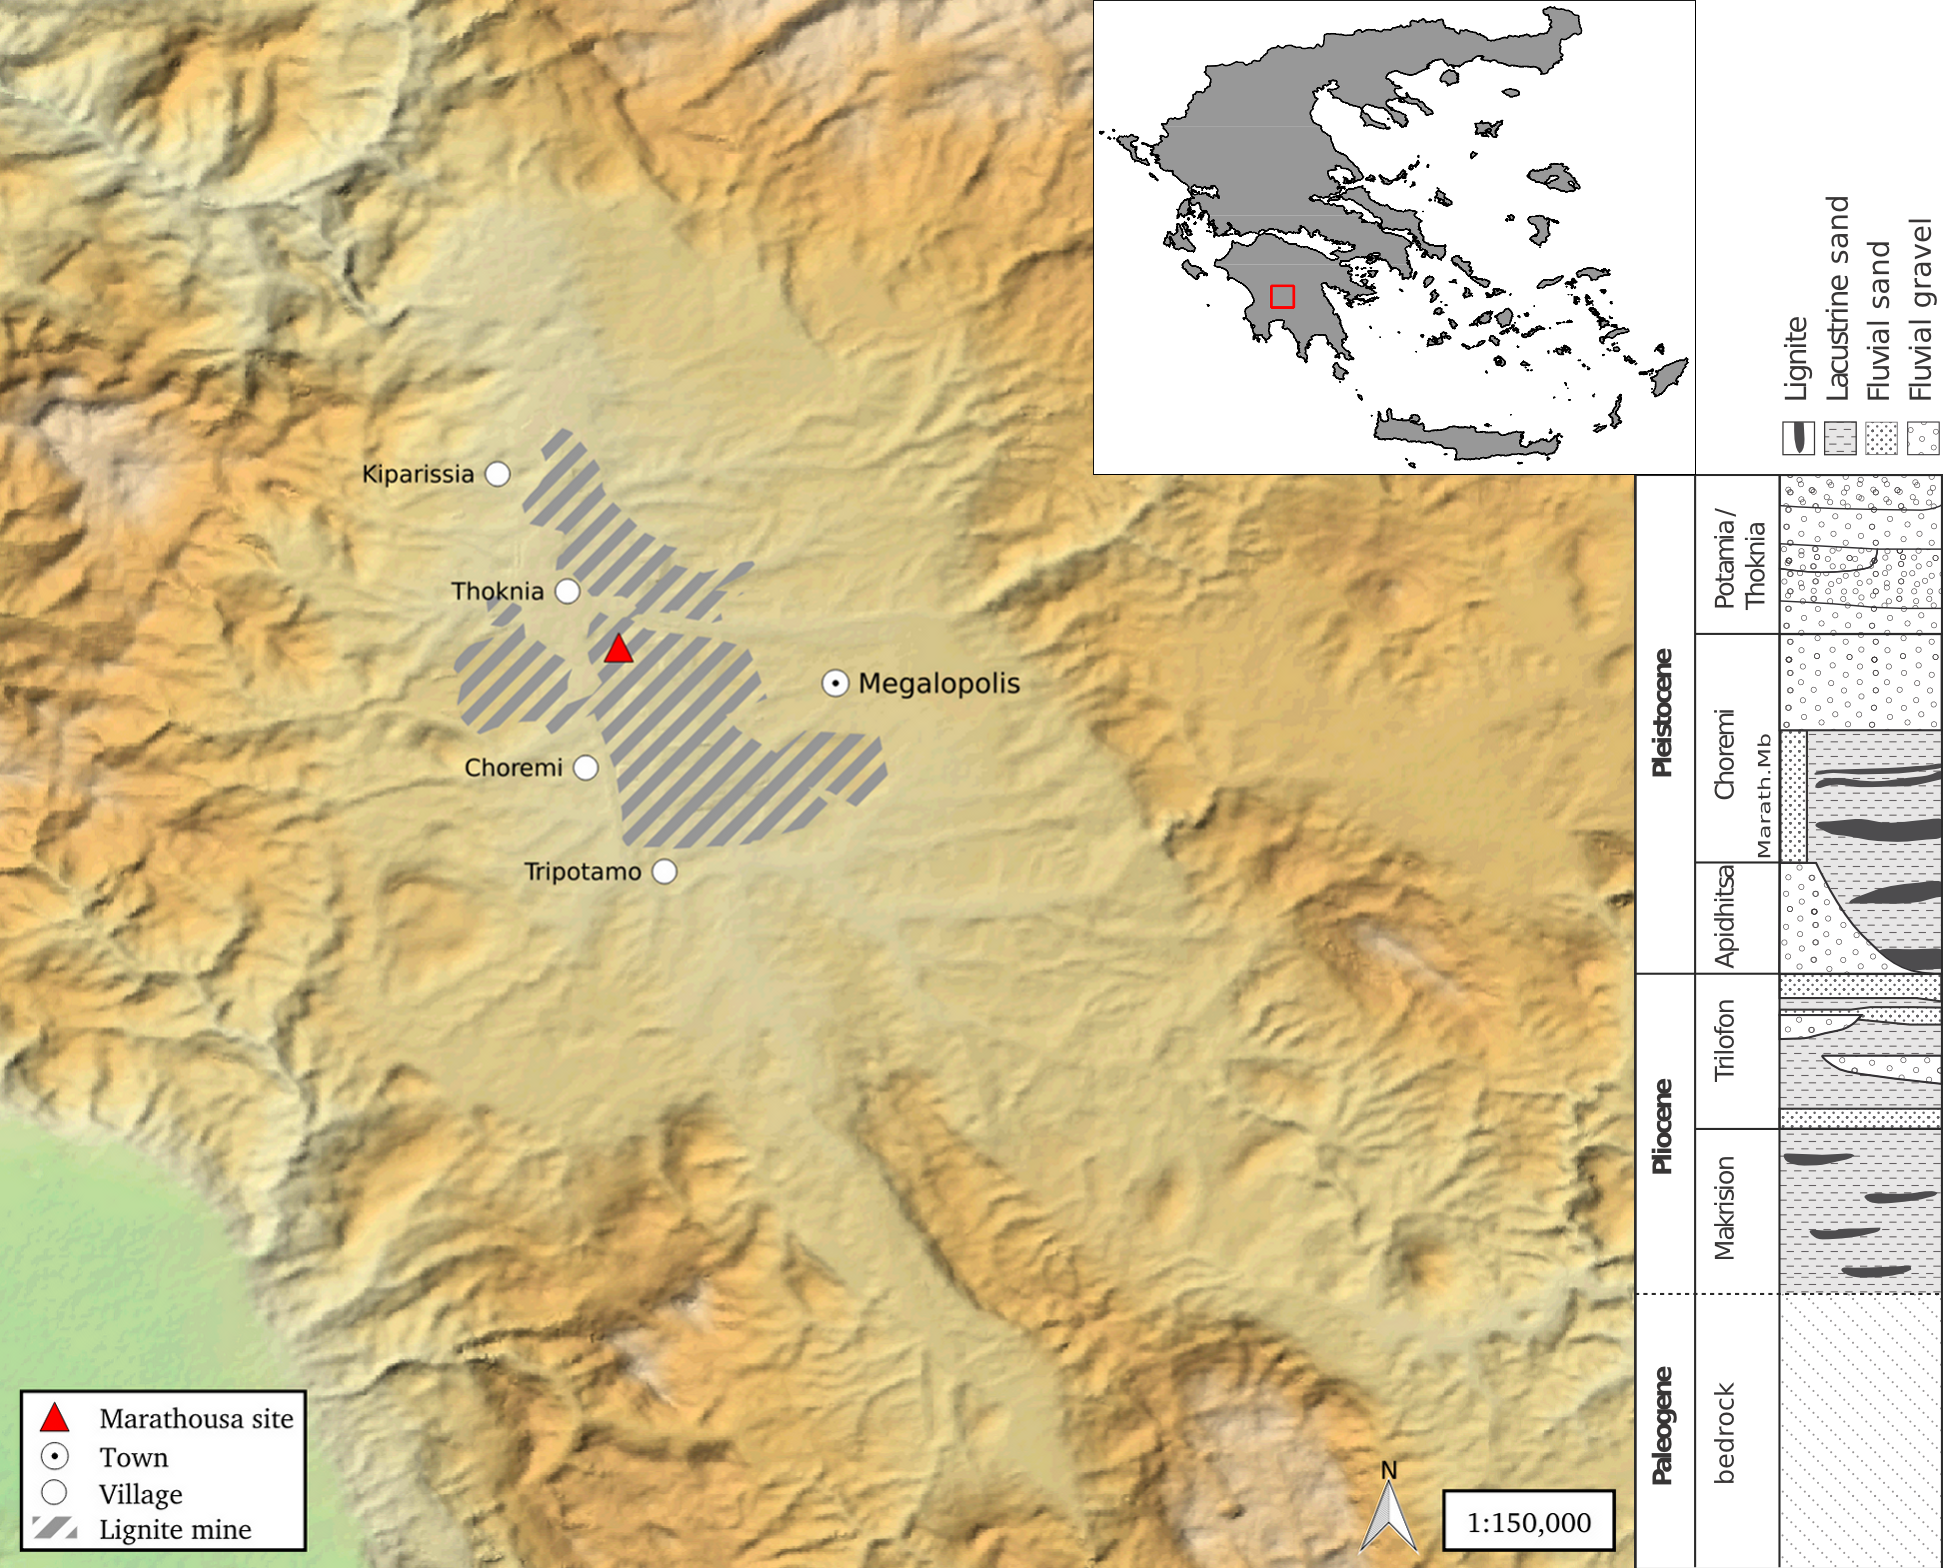
\includegraphics[width=1\textwidth]{../manuscript/artwork/Fig1.png}
  \caption{Geographical location of the Marathousa~1 site in the Megalopolis basin and stratigraphic column of the basin, modified after \cite{Vugt2000}.}
  \label{fig:1}
\end{figure*}

%% Archaeological material
Two excavation areas have been investigated since 2013 (Fig.~\ref{fig:2}): Area A, where several skeletal elements of a single individual of \emph{Palaeoloxodon antiquus} have been unearthed, together with a number of lithic artefacts and other faunal remains; and Area B, located 60 m to the South along the exposed section, where the lithic assemblage is richer and occurs in association with a faunal assemblage composed of isolated elephant bones, cervids and carnivores among others. Bones from Area B are characterized by a high degree of fragmentation (bone fragments make up 93.4\% of the assemblage), with their maximal diameter mostly measuring less than 80mm \citep{Konidaris,Tourloukis}. Evidence of butchering (cut-marks) have been identified on two of the elephant bones from Area A, as well on elephant and other mammal bones from Area B \citep{Konidaris}.

\begin{figure*}[]
  \centering
  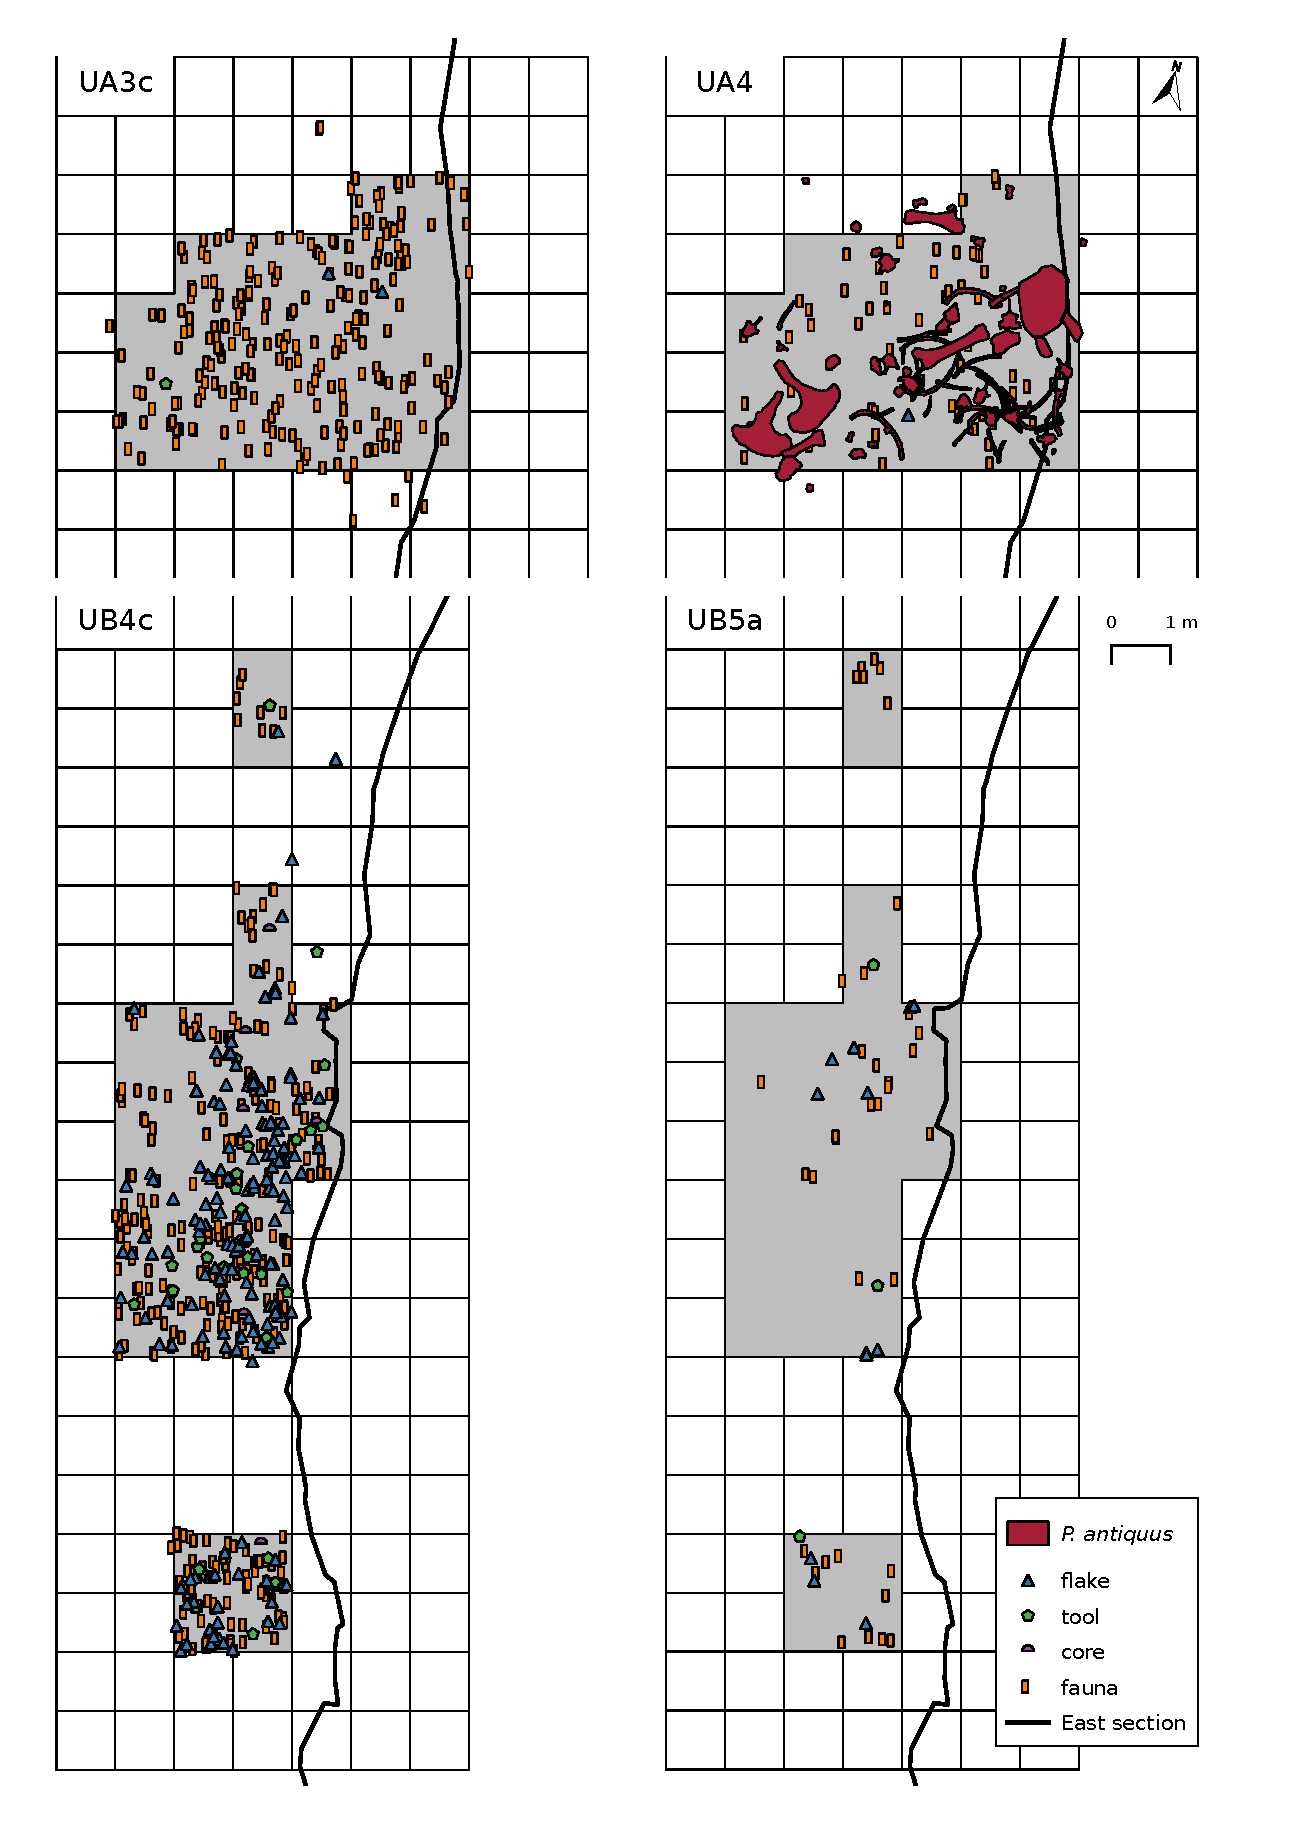
\includegraphics[width=.9\textwidth]{../manuscript/artwork/Fig2.pdf}
  \caption{Distribution maps of the plotted remains from areas A (units UA3c and UA4) and B (units UB4c and UB5a), collected until 2015. Due to their high number, lithic debris/chips are not plotted. The plotted remains of the \emph{P. antiquus} skeleton were collected until 2016. Grey zones mark the 2013-2015 excavation areas. Area B is located 60 m to the South, along the exposed East section of the lignite quarry.}
  \label{fig:2}
\end{figure*}

%% Stratigraphic framework
The sedimentary sequence of the site (Fig.~\ref{fig:3}) includes lacustrine and fluvio-lacustrine clastic deposits sandwiched between two lignite seams (UA7-UB10 and UA1-UB1) \citep{Karkanas}. A major hiatus (contacts between UA3 and UA4, and between UB5 and UB6), attributed to exposure and erosion of a lake shore mudflat, divides the sequence in two parts. The lower part is characterised by relatively high rate sub-aqueous sedimentation of bedded sands and silts, containing low organic and carbonate content. The upper one is characterised by a series of erosional bounded depositional units, attributed to sub-aerial originated organic- and carbonate-rich mud flows and hyperconcentrated flows deposited at the margin of a swamp \citep{Karkanas}.

\begin{figure*}[]
  \centering
  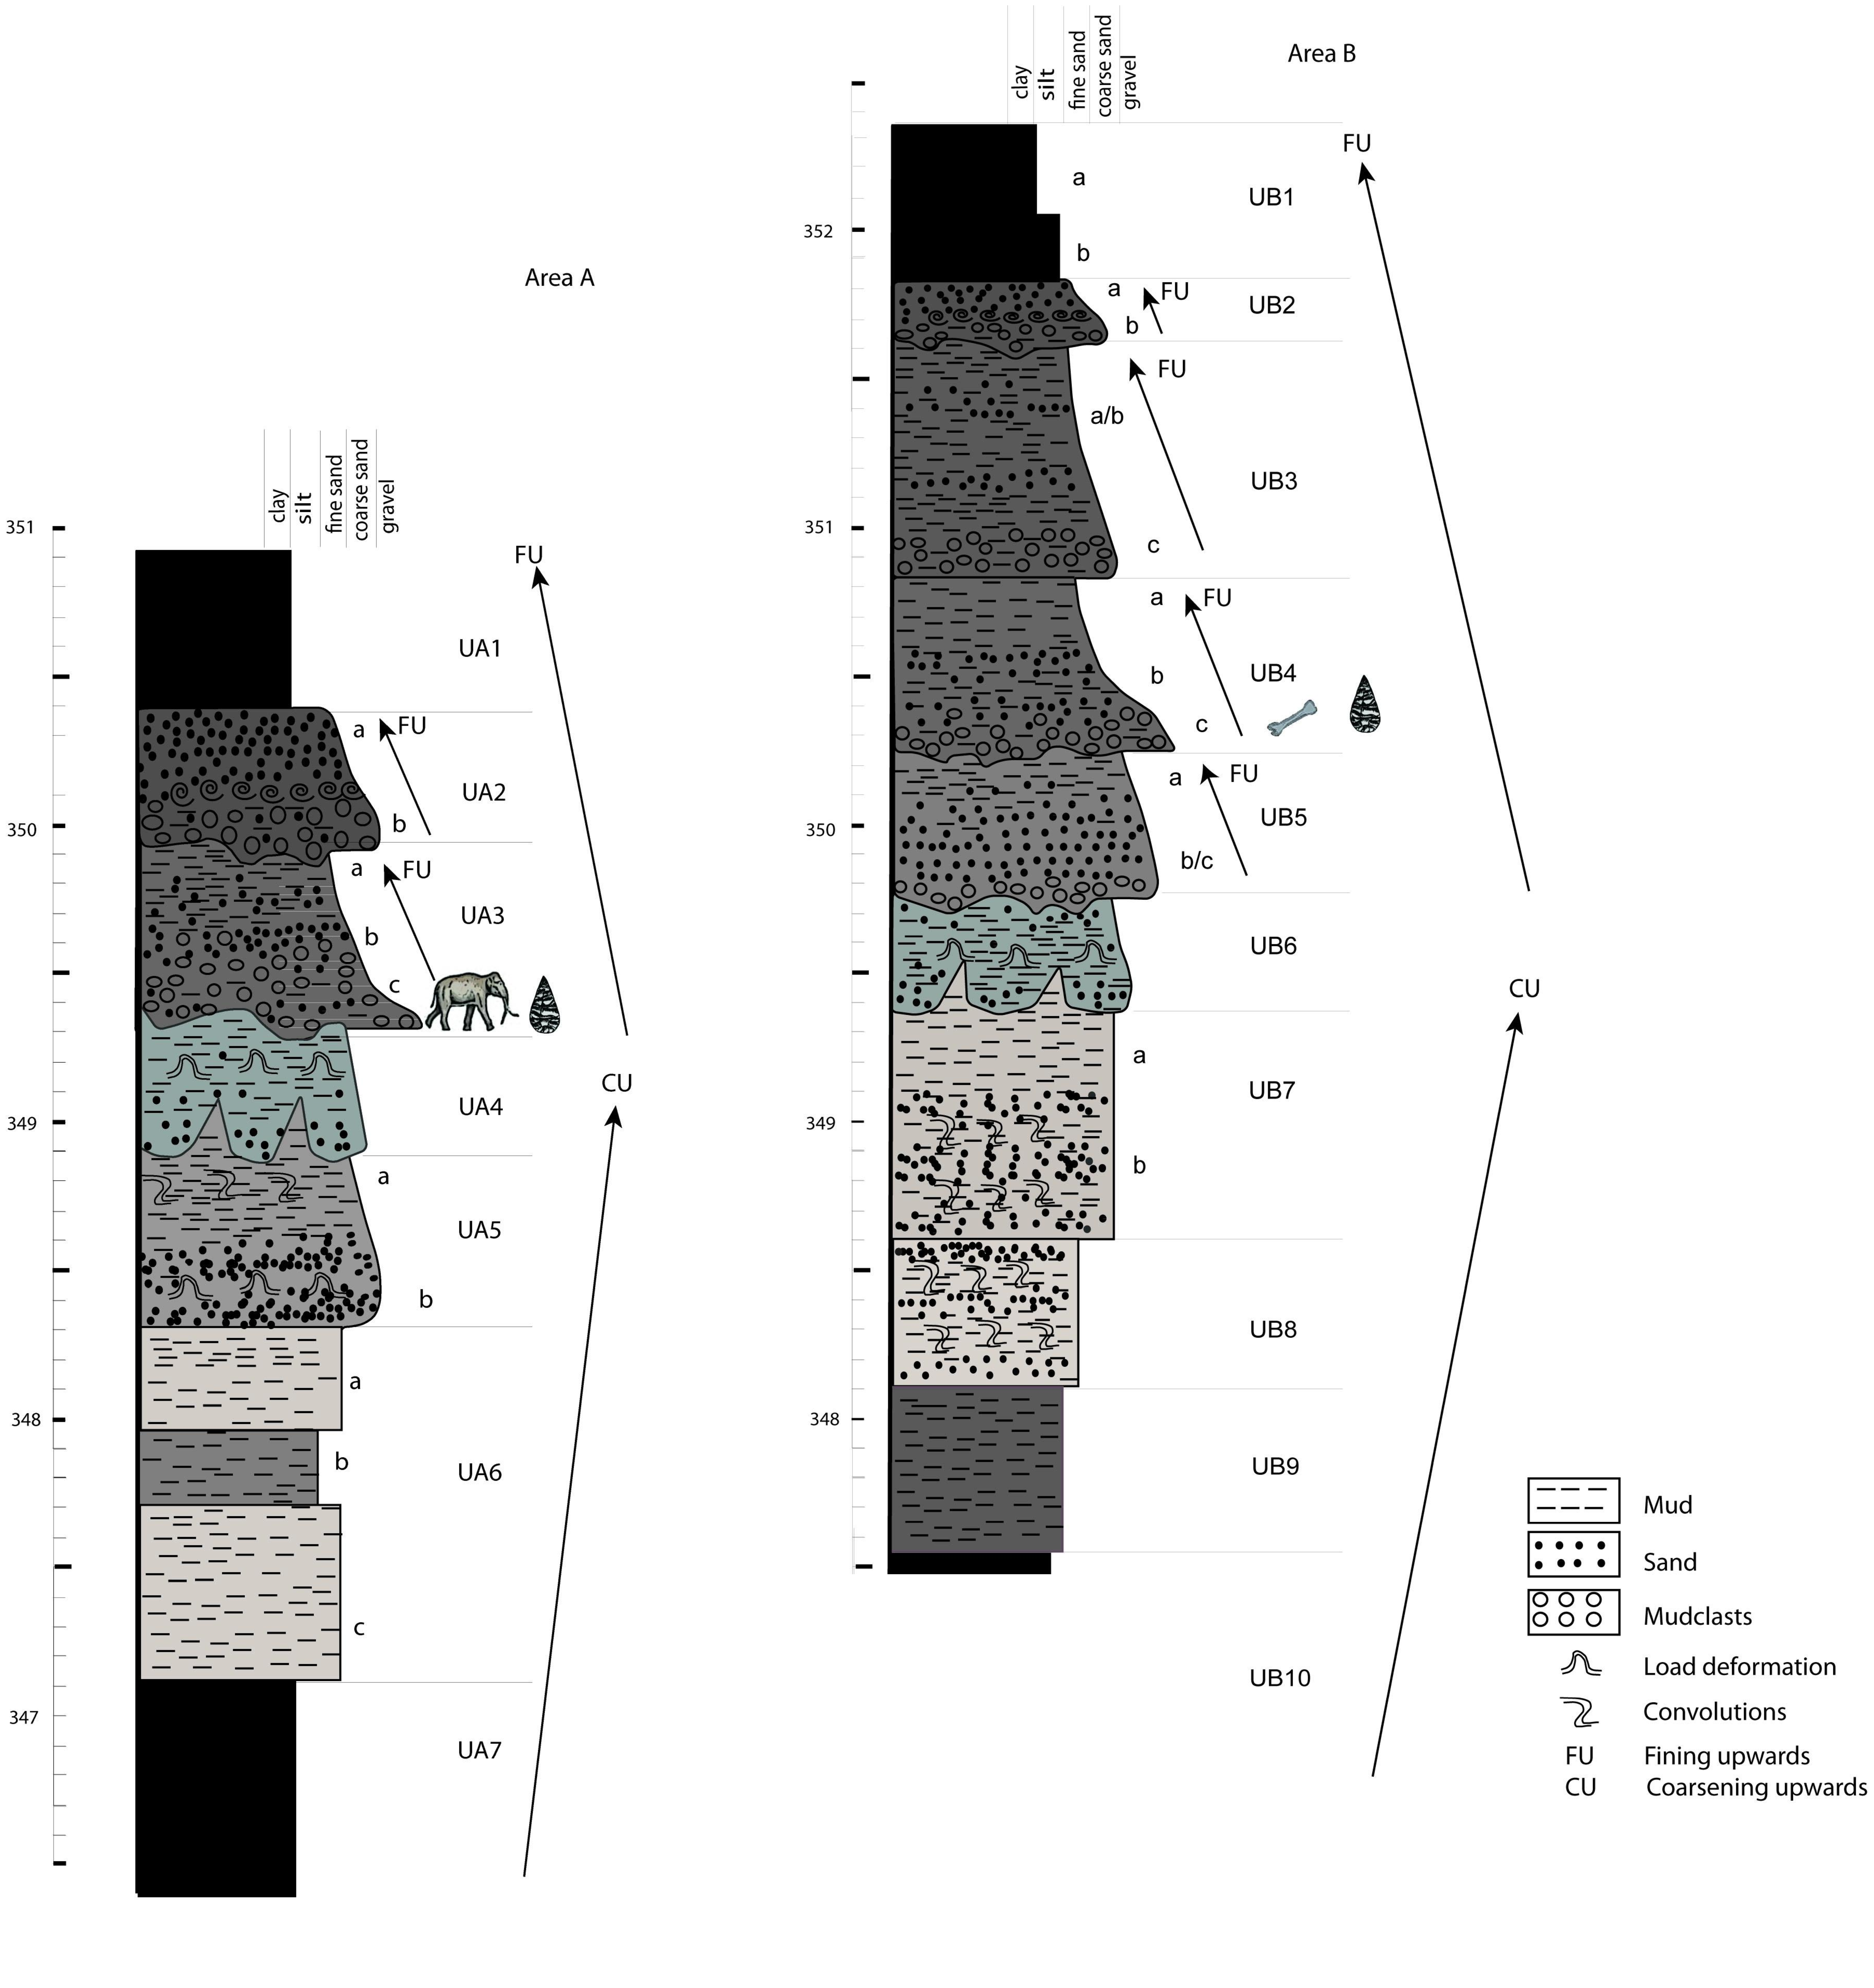
\includegraphics[width=1\textwidth]{../manuscript/artwork/Fig3.pdf}
  \caption{Stratigraphic setting of the Marathousa~1 site, modified after \cite{Karkanas}. Absolute elevations in m~a.s.l.}
  \label{fig:3}
\end{figure*}

The erosional contacts UA3c/4 and UB4c/5a separate the two main find-bearing units in both areas (Fig.~\ref{fig:3}). In Area A, the elephant remains lie at the contact of UA3c/4 and are covered by UA3c (Fig.~\ref{fig:4}a); while in Area B, most of the remains were collected from unit UB4c (Figs.~\ref{fig:2} and ~\ref{fig:4}b). Units UA3c and UB4c (organic- and intraclast-rich silty sands) resemble dilute mud flows, showing a chaotic structure of rip-up clasts from the underlying unit, small-to-large wood fragments and rare rock clasts. In Area B, a relatively low number of remains was also found in massive organic-rich silty sands (UB5a, Fig.~\ref{fig:2}), which locally overlay channelised sands (UB5b/c), probably not preserved in Area A \citep{Karkanas}.

\begin{figure*}[]
  \centering
  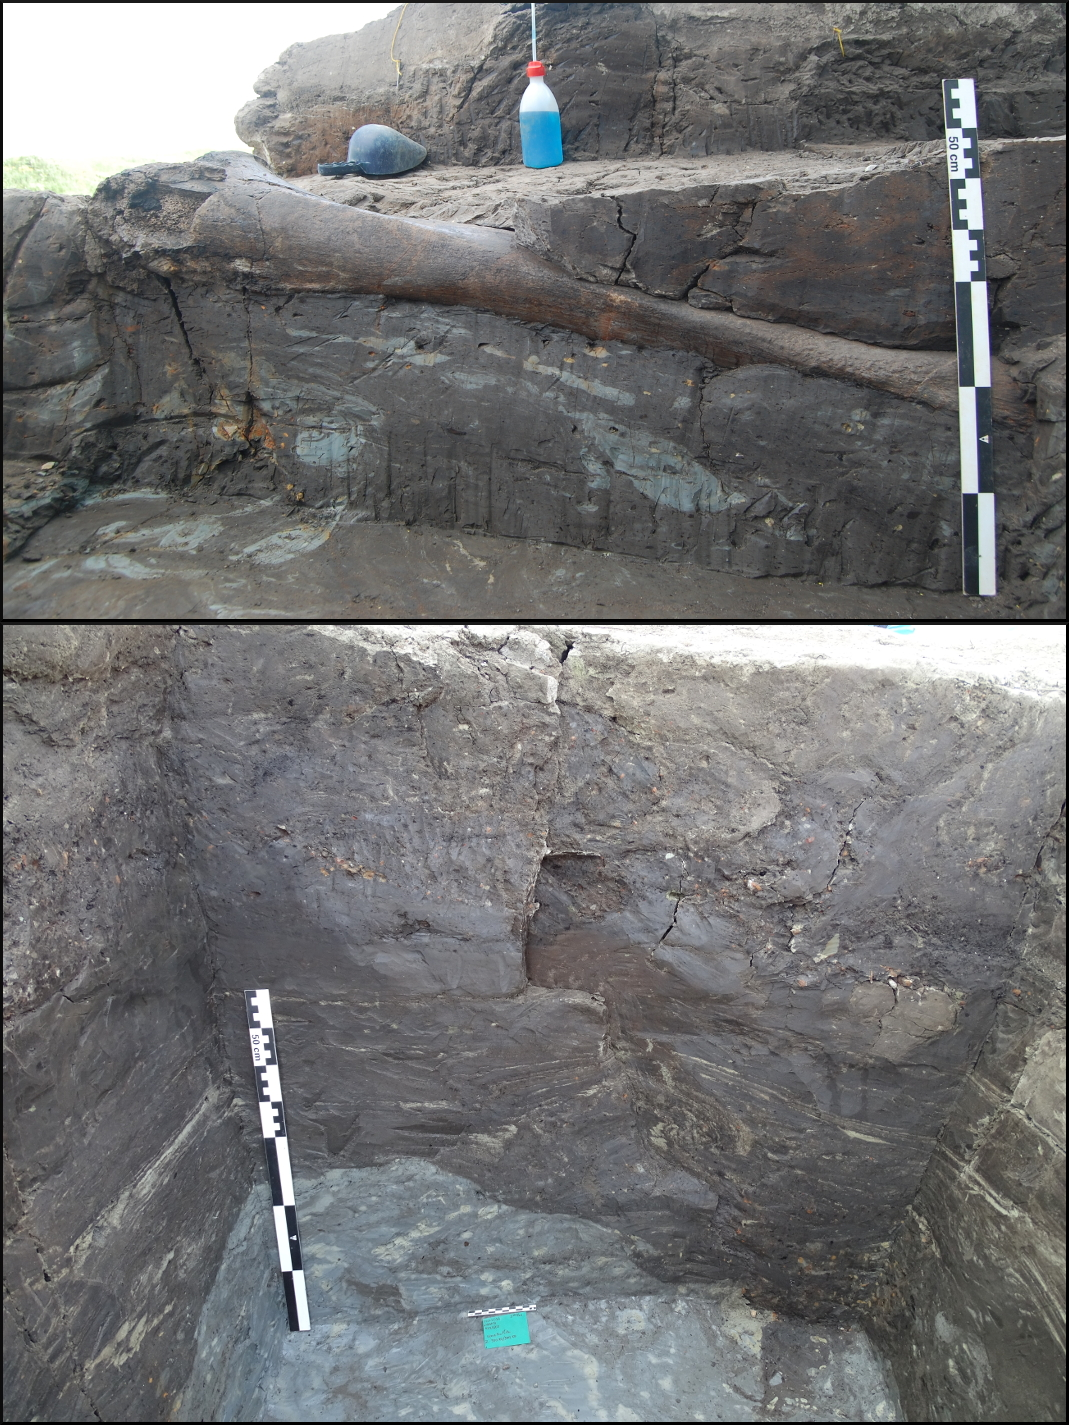
\includegraphics[width=0.5\textwidth]{../manuscript/artwork/Fig4.png}
  \caption{Photograph (2017) of the left femur of the \emph{P. antiquus} skeleton, lying at the UA3c/4 contact and covered by unit UA3c (a). West profile (2014) of the excavation Area B (square 932/603), exposing the UB4c/5a (black solid line) and the UB5/6 erosional contacts (b).}
  \label{fig:4}
\end{figure*}

%% Main research question!
The flow event described above (units UA3c and UB4c), and specifically the erosional contacts between the fossiliferous horizons in the two areas (UA3c/4 and UB4c/5a), provide the essential background for the analysis and interpretation of the spatial distributions at Marathousa~1. The secondary depositional nature of the main find horizons raises the question of how reliable is the spatial association between the lithic artefacts and the partial skeleton of a single \emph{Palaeoloxodon antiquus} individual and other faunal remains. Since spatial association does not necessarily imply causation, and consequently synchrony, the answer has important consequences for the interpretation of the site in the broader context of the Middle Pleistocene human-proboscidean interactions. We aim to tackle this question and disentangle the formation processes acting at Marathousa~1 on the basis of spatial patterns through a three-prong spatial analytic approach:
\begin{enumerate}
\item By analysing, in a frame of references, the orientation patterns of remains from relevant stratigraphic units;
\item By quantifying and comparing their relative vertical distributions;
\item By identifying spatial trends in either the assemblage intensities and the associations between classes of remains.
\end{enumerate}

%% Hypothesis testing
Two contrasting models of deposition are tested: the autochthonous hypothesis \citep[\emph{sensu}][]{Fernandez-Lopez1991,Dominguez-Rodrigo2012} states that the flow event, represented by units UA3c and UB4c, eroded and scoured the exposed surface (where the elephant was lying), thereby entraining clastic material (including artefacts) and re-depositing \citep[\emph{sensu}][]{Fernandez-Lopez1991} this material at a close distance. This model implies the loss of any original, pristine spatial relations between remains, but minor transport from the primary depositional \emph{loci}. On the other hand, the allochthonous hypothesis \citep[\emph{sensu}][]{Fernandez-Lopez1991,Dominguez-Rodrigo2012} implies significant transport from the original \emph{loci} of deposition and re-elaboration \citep[\emph{sensu}][]{Fernandez-Lopez1991}. According to this model, the spurious spatial association between the lithic artefacts and faunal remains does not support any behavioural interpretation.

\section{Material and methods}

%% Excavation protocol
Since 2013, systematic investigation of the Marathousa~1 site has been carried out by a joint team from the Ephoreia of Palaeoanthropology-Speleology (Greek Ministry of Culture) and the University of Tübingen. A grid system of 1 square meter units was set up, oriented -14 degrees off the magnetic North, and including the two areas of investigation. The excavation of the deposit proceeded in 50x50~cm sub-squares in Area B and 1x1~m squares in Area A, and spits of 5 to 10~cm thickness, respectively. Systematic water-screening of sediments was carried out on-site using 1~mm sieves in order to guarantee recovery of the small-size fraction (e.g., micro-artefacts, small mammal remains, fish, molluscs and small fragments of organic and inorganic material). The three-dimensional coordinates of finds (i.e., all the lithic artefacts, teeth and diagnostic bones; bones and organic material with a-axis $\geq20$~mm), collected spits of sediment, samples and geological features (e.g., erosional contacts and mud cracks) were recorded with a total station. Specifically, the three-dimensional position of the finds was always recorded at the lowest point of contact of the item with the sediment. Dense clouds of surface points of the elephant skeletal elements were acquired using both a total station and a close-range photogrammetric technique.

The dimensions (length, width and thickness) of registered finds were measured on-site with millimetre rules. Orientation (plunge and bearing) of elongated particles (i.e., faunal remains, large wood fragments and lithic artefacts) was recorded since 2013 using a clock-like system (the bearing was measured, relatively to the grid North, in twelve clockwise intervals of 30°; the plunge with a 22.5° accuracy). In 2015, the use of a compass and inclinometer with an accuracy of 1° was introduced in Area B to gradually replace the former method.

The widespread use of a compass and inclinometer to record orientation data \citep[][among others]{Voorhies1969,Fiorillo1991,Bertran1995,Bertran1997,Lenoble2004,Eberth2007,Eren2010,Benito-Calvo2011a,Dominguez-Rodrigo2012,Dominguez-Rodrigo2013,Dominguez-Rodrigo2014,Cobo-Sanchez2014,Organista2017} was favoured over the alternative use of a total station \citep[][among others]{Kluskens1990,Dibble1997,McPherron2005,Enloe2006,Bernatchez2010}, mostly due to the time-restricted conditions of the rescue excavation conducted at Marathousa~1.

Measurements of the bearing (azimuth) and plunge (dip) of elongated finds were taken along the symmetrical longitudinal a-axis (SLA) of elongated bones \citep{Dominguez-Rodrigo2013}, lithic artefacts \citep{Bertran1995} and wood fragments \citep{Macdonald1985}, using the lowest endpoint of the a-axis as an indicator of the vector direction.

Other major axes have been alternatively used with the recent application of GIS techniques to retrieve orientation data from secondary source, i.e., from excavation photographs, drawings or maps \citep{Boschian2010,Benito-Calvo2011,Torre2013a,Walter2013,Garcia-Moreno2016,Sanchez-Romero2016}. However, the experimental works of \cite{Dominguez-Rodrigo2013} and \cite{Dominguez-Rodrigo2014} showed that the SLA, defined as the major axis which symmetrically divide the bone, is more accurate in estimating the flow direction, regardless of bone shape. This a-axis is widely used in taphonomic studies \citep[][among others]{Toots1965,Voorhies1969,Eberth2007,Dominguez-Rodrigo2012,Dominguez-Rodrigo2014c,Aramendi2017} for determining the preferential orientation of anisotropic assemblages. The a-axis or major axis of the artefact, measured as the long diameter of the triaxial ellipsoid that approximates the particle shape \citep{Krumbein1941}, is as well used in studies which employ a sedimentological approach to archaeological fabric \citep[][among others]{Bertran1995,Bertran1997,Lenoble2004,Benito-Calvo2009}.

%% Material/areas object of analysis
The present study focuses on the excavated stratigraphic units in which most of the archaeological and palaeontological remains were recovered in both excavation areas, namely in UA3c and UA4 in Area A, and UB4c and UB5a in Area B. From the total, subset samples of material were used for each specific spatial analysis. For the fabric analysis we included material collected until 2016. For the vertical distribution and point pattern analyses, the region of investigation was limited to the squares excavated from 2013 until 2015, 25 and 29 square meters respectively in each area (Fig.~\ref{fig:2}).

%% Reproducible research
The analyses were performed in \textsf{R} statistical software \citep{RCoreTeam2017}. In order to make this research reproducible \citep{Marwick2017,Marwick2017a}, a repository containing a compendium of data, source code and text is open licensed and available at the DOI: \href{https://doi.org/10.5281/zenodo.822272}{10.5281/zenodo.822272}

\subsection{Fabric analysis}

%% Intro
The taphonomic study of the orientation pattern of elongated sedimentary particles, including bones and artefacts, first addressed by \cite{Voorhies1969,Isaac1967,Bar-Yosef1972,Schick1986}, more recently led to a noteworthy development of methods and propagation of applications in Palaeolithic site formation studies \citep[][among others]{Bertran1995,Bertran1997,Lenoble2004,Lenoble2008,McPherron2005,Benito-Calvo2009,Benito-Calvo2011a,Benito-Calvo2011,Bernatchez2010,Boschian2010,Dominguez-Rodrigo2012,Dominguez-Rodrigo2013,Dominguez-Rodrigo2014,Torre2013a,Walter2013,Garcia-Moreno2016,Sanchez-Romero2016}.

Fabric analysis can provide valuable insight into site formation and taphonomic processes, allowing discrimination between different orientation patterns (isotropic, linear or planar) possibly associated with a range of sedimentary processes. Whereas water-flow deposits are generally characterised by relatively good sorting and preferred orientation of clasts parallel, or normal to the flow direction (linear fabric) \citep{Petraglia1994}; debris-flow deposits mostly exhibit massive, poorly bedded mixtures of unsorted sediments and random orientation of clasts (isotropic fabric), except at the flow margins where linear fabric may occur \citep{Pierson2005}. On the other hand, undisturbed archaeological sites, as well as experimental assemblages, have been observed to have planar fabric \citep{Bertran1997,Lenoble2004}. Nevertheless, grey zones exist between depositional processes, so that an unequivocal discrimination based only on fabric observations is often not possible, and other taphonomic criteria must also be considered \citep{Lenoble2004}. As an example, while overland flows (runoff) have been observed to show some degree of planar fabric \citep{Lenoble2004}, anisotropy without significant transport can be caused in a lacustrine floodplain by low-energy processes such as lake transgression and regression, as well as water-sheet flows formed during rainy seasons \citep{Cobo-Sanchez2014}.

%% Assumptions & Expectations
At the margin of a lacustrine environment, relatively close to the surrounding relief, a combination of high- and low-energy processes can be expected. According to the sedimentological and micromorphological study of the Marathousa 1 site, the main find-bearing horizon is associated with hyperconcentrated flows \citep{Karkanas}. Hyperconcentrated flows are intermediate states, defined by sediment concentration, in the continuum between sub-aerial water flows and debris flows. \cite{Benvenuti2002} reported that, when a turbulent hyperconcentrated flow expands over a surface - as in the case of Marathousa~1 - a two-phase flow may develop, with a more concentrated, coarser grained bottom flow-layer (traction carpet) moving slower than the upper turbulent flow-layer carrying wash-load and suspended load. Resultant deposit may exhibit diagnostic inverse grading, or a continuously aggrading bed. Parallel or normal orientation of the clasts to the flow direction can be observed \citep{Benvenuti2002}. A simulation model also showed that linear fabric can develop in mud flows. However, after deposition, settling of the clasts may affect the fabric to some extent, depending on the viscosity of the mud flow \citep{Lindsay1968}.
 
%% Subsets
As part of our three-prong spatial analytic approach, we conducted comparative fabric analysis with the aim to investigate the dynamics of the depositional processes at Marathousa~1. Since fabric strength has been found to be positively correlated with the shape and size of the clast, for the fabric analysis we subset samples of remains with length $\geq2$~cm and elongation index (the ratio length/width) $I_{e}\geq1.6$ \citep{Lenoble2004}. The samples are listed in Table~\ref{tab:1} and include mostly wood fragments and faunal remains from the four stratigraphic units under investigation. Bones have been found to readily react to water flow and show very early anisotropic patterns \citep{Dominguez-Rodrigo2014}. Flume experiments showed that wood fragments as well tend to align parallel to the current direction \citep{Macdonald1985}. No distinction of skeletal elements was made, both due to the high fragmentation rate of faunal remains in Area B, and because recent experiments showed a similar orientation pattern for different bone shapes \citep{Dominguez-Rodrigo2012,Dominguez-Rodrigo2013}.

The sample of bones belonging to the individual of \emph{P. antiquus} from Area A was analysed separately and included the humerus, ulna, femur and tibia; the atlas, axis and other 16 complete vertebrae or vertebral fragments; 29 complete ribs or rib fragments; 2 calcanea; 4 metatarsals/metacarpals; the pyramidal; the trapezoid and the pelvis. The sample from UB5a was too small (only 7 observations) and was therefore excluded. In order to asses the reliability of the orientation data recorded using the clock method, we separately analysed two sub-samples from unit UB4c, selected from a set of finds recorded using both methods. All the sampled observations are representative of the whole study area.

\begin{table*}[]
  \caption{List of sampled observations for the fabric analysis.}
  \label{tab:1}
  \vspace{0.1in}
%  \centering
  \resizebox{.3\textwidth}{!}{
    \begin{tabular}{lllll}
      \hline
      &      & \multicolumn{3}{c}{Type}                        \\
      \cline{3-5}
      Sample                    & $n$  & Fauna & Wood & Lithic \\
      \hline
      UA3c                      & 49   & 23    & 25   & 1      \\
      UA4                       & 38   & 8     & 30   & -      \\
      \emph{P. antiquus}   & 63   &       &      &        \\
      UB4c                      & 38   & 30    & 1    & 7     \\
      \hline
    \end{tabular}
  }
\end{table*}

%% Methods
Rose diagrams and uniformity tests, such as Rayleigh, Kuiper, Watson and Rao tests \citep{Jammalamadaka2001}, were used to visualise and evaluate circular isotropy in the sample distribution. The Rayleigh test is used to assess the significance of the sample mean resultant length ($\bar{R}$), assuming that the distribution is unimodal and not bi- or plurimodal. The $\bar{R}$ ranges from 0 to 1: values close to 1 indicate that the data are closely clustered around the mean direction; when the data are evenly spread $\bar{R}$ has a value close to 0. A $p-value$ lower than 0.05 rejects the hypothesis of uniformity with a 95\% confidence interval. Kuiper, Watson and Rao are omnibus tests used to detect multimodal departures from circular uniformity. The Kuiper test \citep{Kuiper1960} is a rotation-invariant Kolmogorov-Smirnov test statistic for testing the null hypothesis that the empirical distribution function fits a uniform distribution function. The Watson test \citep{Watson1961} is instead related to the Cramer-von Mises test. The Rao’s spacing test \citep{Jammalamadaka2001} is based on the idea that in a uniform distribution successive observations should be approximately evenly spaced and it tests deviation from this distribution. For all the tests, results are evaluated against critical values: a result higher than the critical value rejects with confidence the null hypothesis. We applied three omnibus tests since none of them have very high power and some studies suggested that there is no test that is superior to the others under all circumstances \citep{Pewsey2013}. 

Randomness testing of three-dimensional data was conducted with the Woodcock $S_1/S_3$ test \citep{Woodcock1983}. Considering both the plunge and bearing of the oriented items, this method, based on three ordered eigenvalues ($S_1$, $S_2$, $S_3$), is able to discriminate the shape and strength of the distributions. The shape parameter $K=\frac{ln(S_1/S_2)}{ln(S_2/S_3)}$ ranges from zero (uni-axial girdles) to infinite (uni-axial clusters). The parameter $C=ln(S_1/S_3)$ expresses the strength of the preferential orientation, and its significance is evaluated against critical values from simulated random samples of different sizes. A perfect random uniform distribution would have $C=0$ and $K=1$.

The Benn diagram \citep{Benn1994} adds to the Woodcock test an isotropy ($IS=S_3/S_1$) and an elongation ($ES=1-(S_2/S_1)$) index. Like the former method, it is able to differentiate between linear (cluster), planar (girdle) or isotropic distributions. There are no published raw data from actualistic studies on hyperconcentrated flows or other depositional processes affecting the orientation of bones and artefacts deposited on lacustrine floodplains (but see \cite{Morton2004} and \cite{Cobo-Sanchez2014} as pioneer studies on this subject). However, we included in the Benn diagram relevant references to published results from observation of fabrics in modern subaereal slope deposits, i.e., debris flow and runoff \citep{Bertran1997,Lenoble2004}.

\subsection{Vertical distribution}

%% Intro
The vertical distribution of materials has been long investigated with the aim of identifying cultural levels, by visually interpreting cross-sectional plots. However, recent advances in GIS techniques allow to inspect at higher resolution the three-dimensional distributions of archaeological remains \citep[][among others]{McPherron2005a,Anderson2008}.

%% Assumptions & Expectations
In analysing the vertical dispersion of material at Marathousa~1, we provisionally assume that a general concentration of unsorted lithic artefacts and faunal remains in the proximity of the erosional surfaces would support an autochthonous origin of the assemblages; whereas a homogeneous vertical distribution of remains from the UA3c and UB4c units would suggest an allochthonous origin, significant transport and subsequent re-deposition of the material. Indeed, massive process such as hyperconcentrated flows, have high erosional power and rather chaotic structure, which may result in inverse or normal grading \citep{Benvenuti2002}.

%% Subsets
In order to estimate the degree of vertical dispersion while controlling for the size of the archaeological material, dimensional classes were set up following typological criteria. Lithic artefacts were classified as debris/chips when smaller than a cutoff length of 15~mm \citep{Tourloukis}. Other classes include flakes, tools and cores; the latter being the bigger and heavier debitage product. Table~\ref{tab:2} summarises the sample size for each class. Lithic debris/chips constitute the larger part of the assemblage from UB4c (60\%) and UB5a (49\%); whereas in Area A they represent only a moderate percentage in the upper UA3c unit (16\%). The very rare presence of lithic artefacts in the underlying unit UA4 is nevertheless significant. In this unit, the faunal remains are also found in much lower numbers, their number reduced to one fourth of those found in UA3c. For the point pattern analysis (see below), we used the same subset of material for both excavation areas.

\begin{table*}[]
  \caption{List of sampled observations for the vertical distribution and point pattern analyses.}
  \label{tab:2}
  \vspace{0.1in}
%  \centering
  \resizebox{.5\textwidth}{!}{
    \begin{tabular}{llllllllllll}
      \hline
      &      & \multicolumn{6}{c}{Lithic class} & \multicolumn{3}{c}{Faunal class} \\
      \cline{3-11}
      Sample         & $n$       & Debris/chip & Flake & Bone flake & Tool & Core & Indet. & Bone & Tooth & Microfauna  \\
      \hline
      UA3c           & 279        & 46         & 2     & -          & 1    & -    & 1      & 171  & 14    & 44          \\
      UA4            & 61         & 3          & 1     & -          & -    & -    & -      & 45   & 4     & 8           \\
      UB4c           & 1243       & 753        & 154   & 1          & 34   & 6    & 2      & 246  & 28    & 19          \\
      UB5a           & 101        & 50         & 12    & -          & 3    & -    & -      & 30   & 3     & 3           \\
      \hline
    \end{tabular}
  }
\end{table*}

%% Methods
For Area B, the material recovered from the water-screening was randomly provenanced according to the 5~cm depth of the excavated spit and the coordinates of the 50x50~cm quadrant of the excavation square. Following the same excavation protocol, the same procedure was applied for the water-screened material of Area A, which was randomly provenanced according to 3D-coordinates of the 1x1~m excavation square and 10~cm spit.

Since the merely projection of points to virtual profiles is not a suitable method of analysis in presence of erosional, and thus uneven, geological contacts - such as those at Marathousa 1, ordinary Kriging interpolation of the recorded points of contact between the UA3c/UA4 and the UB4c/UB5a stratigraphic units were used to reconstruct the UA3c/4 and UB4c/5a erosional surfaces (Fig.~\ref{fig:5}a,b). In geostatistics, Kriging is a method of interpolation which, from a modelled function of spatial autocorrelation between known points (e.g., recorded elevations), calculates values of unknown points (e.g., predicted elevations). Thus, in order to address our specific objective, i.e., to quantify and analyse the vertical distribution of the archaeological and palaeontological material, we measured the minimum orthogonal distance (d) of each specimen to the interpolated erosional surface (Fig.~\ref{fig:5}c). For the units above and below this surface (i.e., UB4c and UB5a), the relative distribution of lithic classes and faunal remains was informally tested by means of density estimations.

In Area A, the UA3c/4 erosional contact is locally sharp, but, in contrast to Area B, parts of the eroded unit UA4 are mixed with pockets of the UA3c organic-rich silty sands and intraclast-rich mud flows \citep{Karkanas}. However, from sparse known points of the erosional contact, the UA3c/4 surface was interpolated and the vertical dispersion of remains estimated as well. The elephant remains were excluded from this analysis, since they clearly lie horizontally at the UA3c/4 contact (Fig.~\ref{fig:4}a). Finally, a Student's two sample t-test allowed us to compare the empirical distributions of different groups of remains for each stratigraphic unit.

\begin{figure*}[]
  \centering
  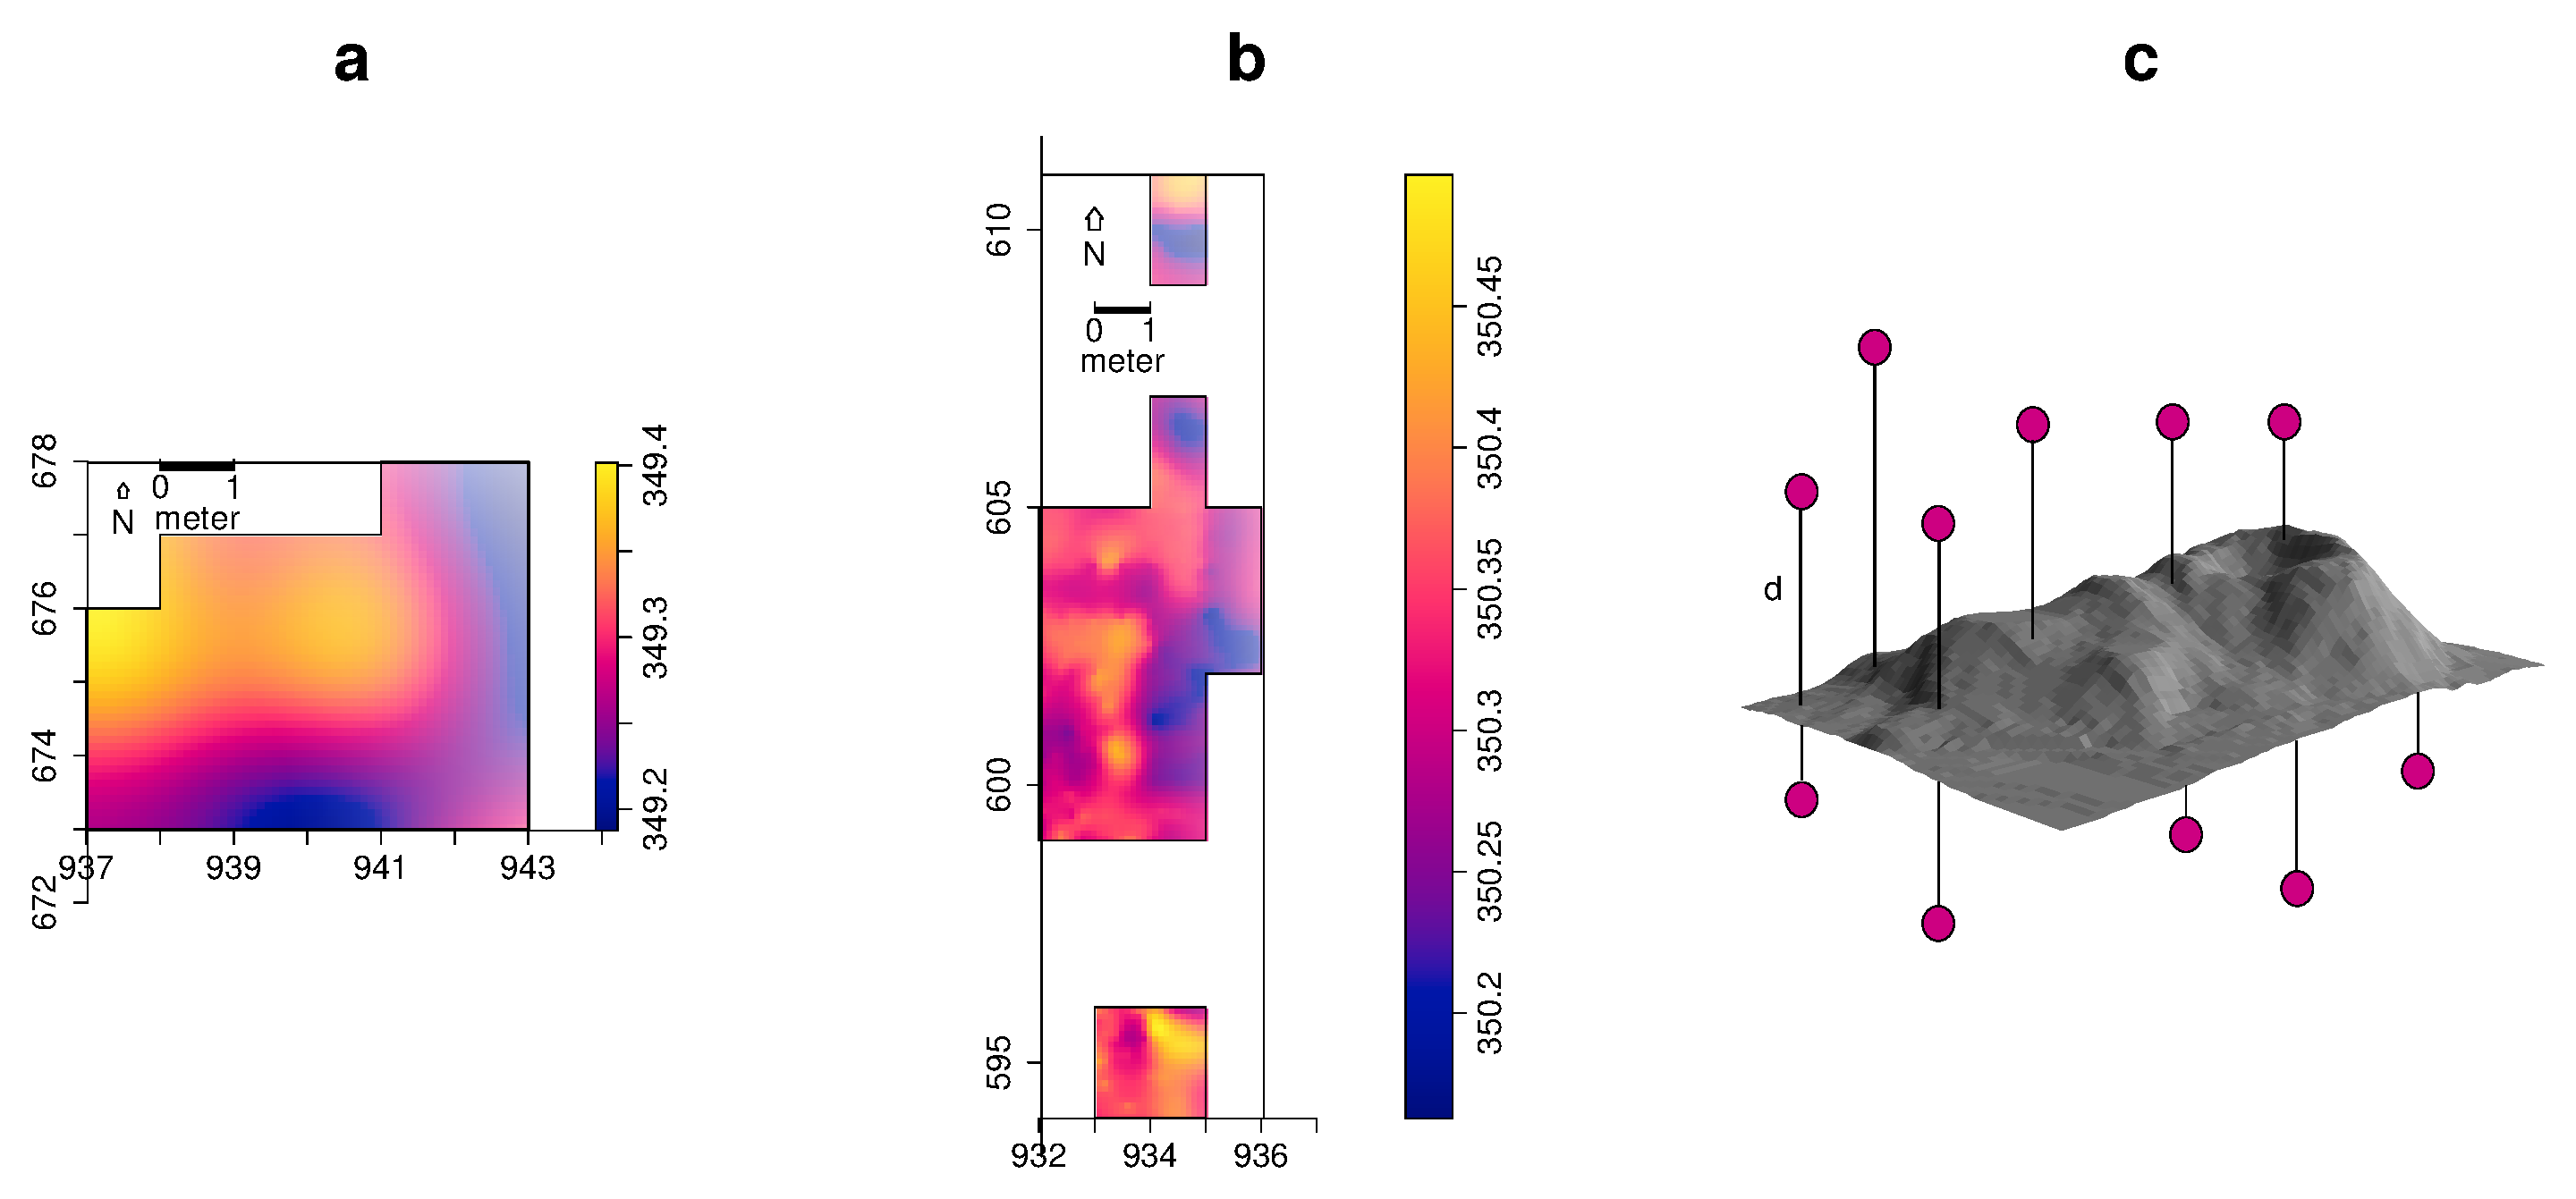
\includegraphics[width=1\textwidth]{../manuscript/artwork/Fig5.pdf}
  \caption{Ordinary Kriging interpolation of the UA3c/4 (a) and UB4c/5a (b) erosional surface; the colour scale denotes absolute elevation in m a.s.l. (c) Illustration of the method used to quantify the vertical dispersion of remains (d) with respect to the UA3c/4 (a) and UB4c/5a (b) surface.}
  \label{fig:5}
\end{figure*}

\subsection{Point pattern analysis}

%% Intro
A spatial point pattern is defined as the outcome of a random spatial point process (repetitions of it would always create a different pattern). The observed patterns of the archaeological and palaeontological remains were treated as manifestations of spatial point processes, i.e., site formation processes. Point pattern analysis investigates the spatial arrangement of points with the aim of identifying spatial trends. In order to integrate the previous studies of the fabric and vertical distributions, we directed our point pattern analysis equally to the intensity of the patterns (the rate of occurrence of the recorded finds) and to the spatial interaction between different types of finds.

%% Methods + Assumptions & Expectations
As the average number of random points per unit area, intensity informs about homogeneity or inhomogeneity in the distribution of events (e.g., clasts) generated by a point process (e.g., mud flow), i.e., whether the rate of occurrence is uniform or spatially varying across the study area. Intensity, usually non-parametrically evaluated by means of kernel density estimation \citep{Diggle1985}, was assessed for the distribution of material from the UB4c, UB5a and UA3c units. Cross-validation bandwidth, which assumes a Cox process, and edge correction were applied using the methods described in \cite{Diggle1985}.

In the presence of a covariate, it is recommended to further investigate the dependence of intensity on that explanatory variable \citep{Baddeley2012}. In order to evaluate whether variation in the density of materials was correlated to the topography of the erosional surface, we computed a local likelihood smoothing estimate of the intensity of remains from UB4c as a function of the UB4c/5a surface elevation model. Formal tests enabled us to assess the evidence of that dependence and to quantify the strength of the covariate. The Kolmogorov-Smirnov test of CSR (Complete Spatial Randomness) and Berman's $Z_2$ statistics were used to test the strength of evidence for a covariate effect. The Receiver Operating Characteristic (ROC) plot, and the area under the ROC curve (AUC), closely related to Berman's $Z_2$ test, measure the magnitude of the covariate effect. AUC values close to 1 or 0 indicate strong discrimination, whereas intermediate values (0.5) suggest no discrimination power.

Intensity, evaluated by means of kernel density maps, although informative and widespread in the literature, nonetheless does not provide sufficient information to reliably infer about site formation processes. Whereas intensity is a first-order property of the point process, multiscale inter-point interaction is measured by second or higher-order moment quantities, such as the Ripley's $K$ correlation function \citep{Ripley1976,Ripley1977} and the distance $G$-, $F$- and $J$-functions. Three different types of inter-point interaction are possible: random, regular or cluster. In a hypothesis-testing framework, point-wise envelopes are computed by a number of random simulations of the null hypothesis (i.e., random/Poisson distribution). Thus, values of the empirical distribution (black solid line) are plotted against the benchmark value (red dotted line) and the envelopes (grey area) which specify the critical points for a Monte Carlo test \citep{Ripley1981}. Regular patterns are assumed to be the result of inhibition processes, while cluster patterns are the result of attraction processes.

In order to test the spatial interaction between remains associated with the erosional event of UB4c and those associated with the underlying UB5a unit, we treated the data as a multivariate point pattern, assuming that the point patterns in UB4c and UB5a are expressions of two different stationary point processes, i.e., depositional events. We performed a cross-type pair correlation function $g_{ij}(r)$, derivative of the multitype $K_{ij}(r)$ function, which is the expected number of points of type $j$ lying at a distance $r$ of a typical point of type $i$. The function is a multiscale measurement of the spatial dependence between types $i$ (UB4c) and $j$ (UB5a). Randomly shifting in 199 Monte Carlo permutations each of the two patterns, independently of each other, estimated values of $\hat{g}_{ij}(r)$ are compared to a benchmark value $g_{ij}(r)=1$, which is consistent with independence or at least with lack of correlation between the two point processes.

In addition to the pair correlation function, the multitype nearest-neighbour $G_{ij}(r)$ function was used to estimate the cumulative distribution of the distance from a point of type $i$ (UB4c) to the nearest point of type $j$ (UB5a). It measures the spatial association between the two assemblages. For the cross-type $G$-function, the null hypothesis states that the points of type $j$ follow a Poisson (random) distribution in addition to being independent of the points of type $i$. Thus, in a randomisation technique, when the solid line of the observed distribution ($\hat{G}_{ij}(r)$ or $\hat{g}_{ij}(r)$) is above or below the shaded grey area, the pattern is significantly consistent with clustering or segregation, respectively. In order to reduce the edge effect bias in estimating the correlation between points, we implemented Ripley's isotropic edge correction \citep{Ohser1983,Ripley1988}.

Complete spatial randomness and independence (CSRI) of the two point processes (UB4c and UB5a) would support an allochthonous origin hypothesis for the assemblage recovered from the UB4c unit. According to the allochthonous model, the massive, chaotic UB4c flow event randomly re-elaborated the material entrained in it, independently from the material deposited in UB5a. On the other hand, positive or negative association can be interpreted as expressions of different autochthonous processes.

As for the three-dimensional distribution of the lithic artefacts in Area A, and their spatial association with the partial skeleton of the \emph{P. antiquus}, we applied three-dimensional univariate and bivariate second-order functions. A rectangular box of 20 square meters and 80~cm vertical extent was selected for the analyses (green outline in Fig.~\ref{fig:11}a). Assuming homogeneity, the univariate pair correlation function $g_3(r)$ was estimated for the pattern of all the artefacts (mostly debris/chips) from UA3c and UA4. In the specific context of the site, complete spatial randomness (CSR) would suggest that the pattern most probably is the result of a random distribution process, such as a high energy mass movement, thus supporting an allochthonous model of deposition. On the other hand, spatial aggregation would support a primary origin of the assemblage. Nevertheless, topography and natural obstructions may generate spatial clustering as well.

In support to the pair correlation function, the cross-type nearest-neighbour function has been applied in order to compute, for each artefact recovered from the UA3c and UA4 units, the nearest point of the three-dimensional clouds of points associated with the elephant skeleton. A prevalence of short distances would indicate aggregation of the lithic artefacts around the mass of the elephant; whereas a uniform or symmetric distribution would support the action of random independent processes.

\section{Results}

\subsection{Fabric analysis}

%% Rose/equal area diagrams & uniformity tests
The rose diagrams in Fig.~\ref{fig:6} visualise the circular distributions of the examined specimens. Overall, the UA4 sample and the sample of elephant bones show unimodal distributions with predominant peaks in the NE quadrant; while the ones from units UA3c and UB4c suggest multimodal distributions. Specifically, the UA4 sample distribution (Fig.~\ref{fig:6}b) spreads largely in the NE quadrant. Similarly, the circular distribution of the elephant sample (Fig.~\ref{fig:6}c), mainly lying in UA4, resembles the former distribution: it is skewed to the SW and concentrated in the NE quadrant. On the other hand, the UA3c sample (Fig.~\ref{fig:6}a) shows a bimodal distribution with two peaks to the E and NE, and the two samples from Area B (Fig.~\ref{fig:6}d,e) suggest a different multimodal scenario uniformly distributed.

\begin{figure*}[]
  \centering
  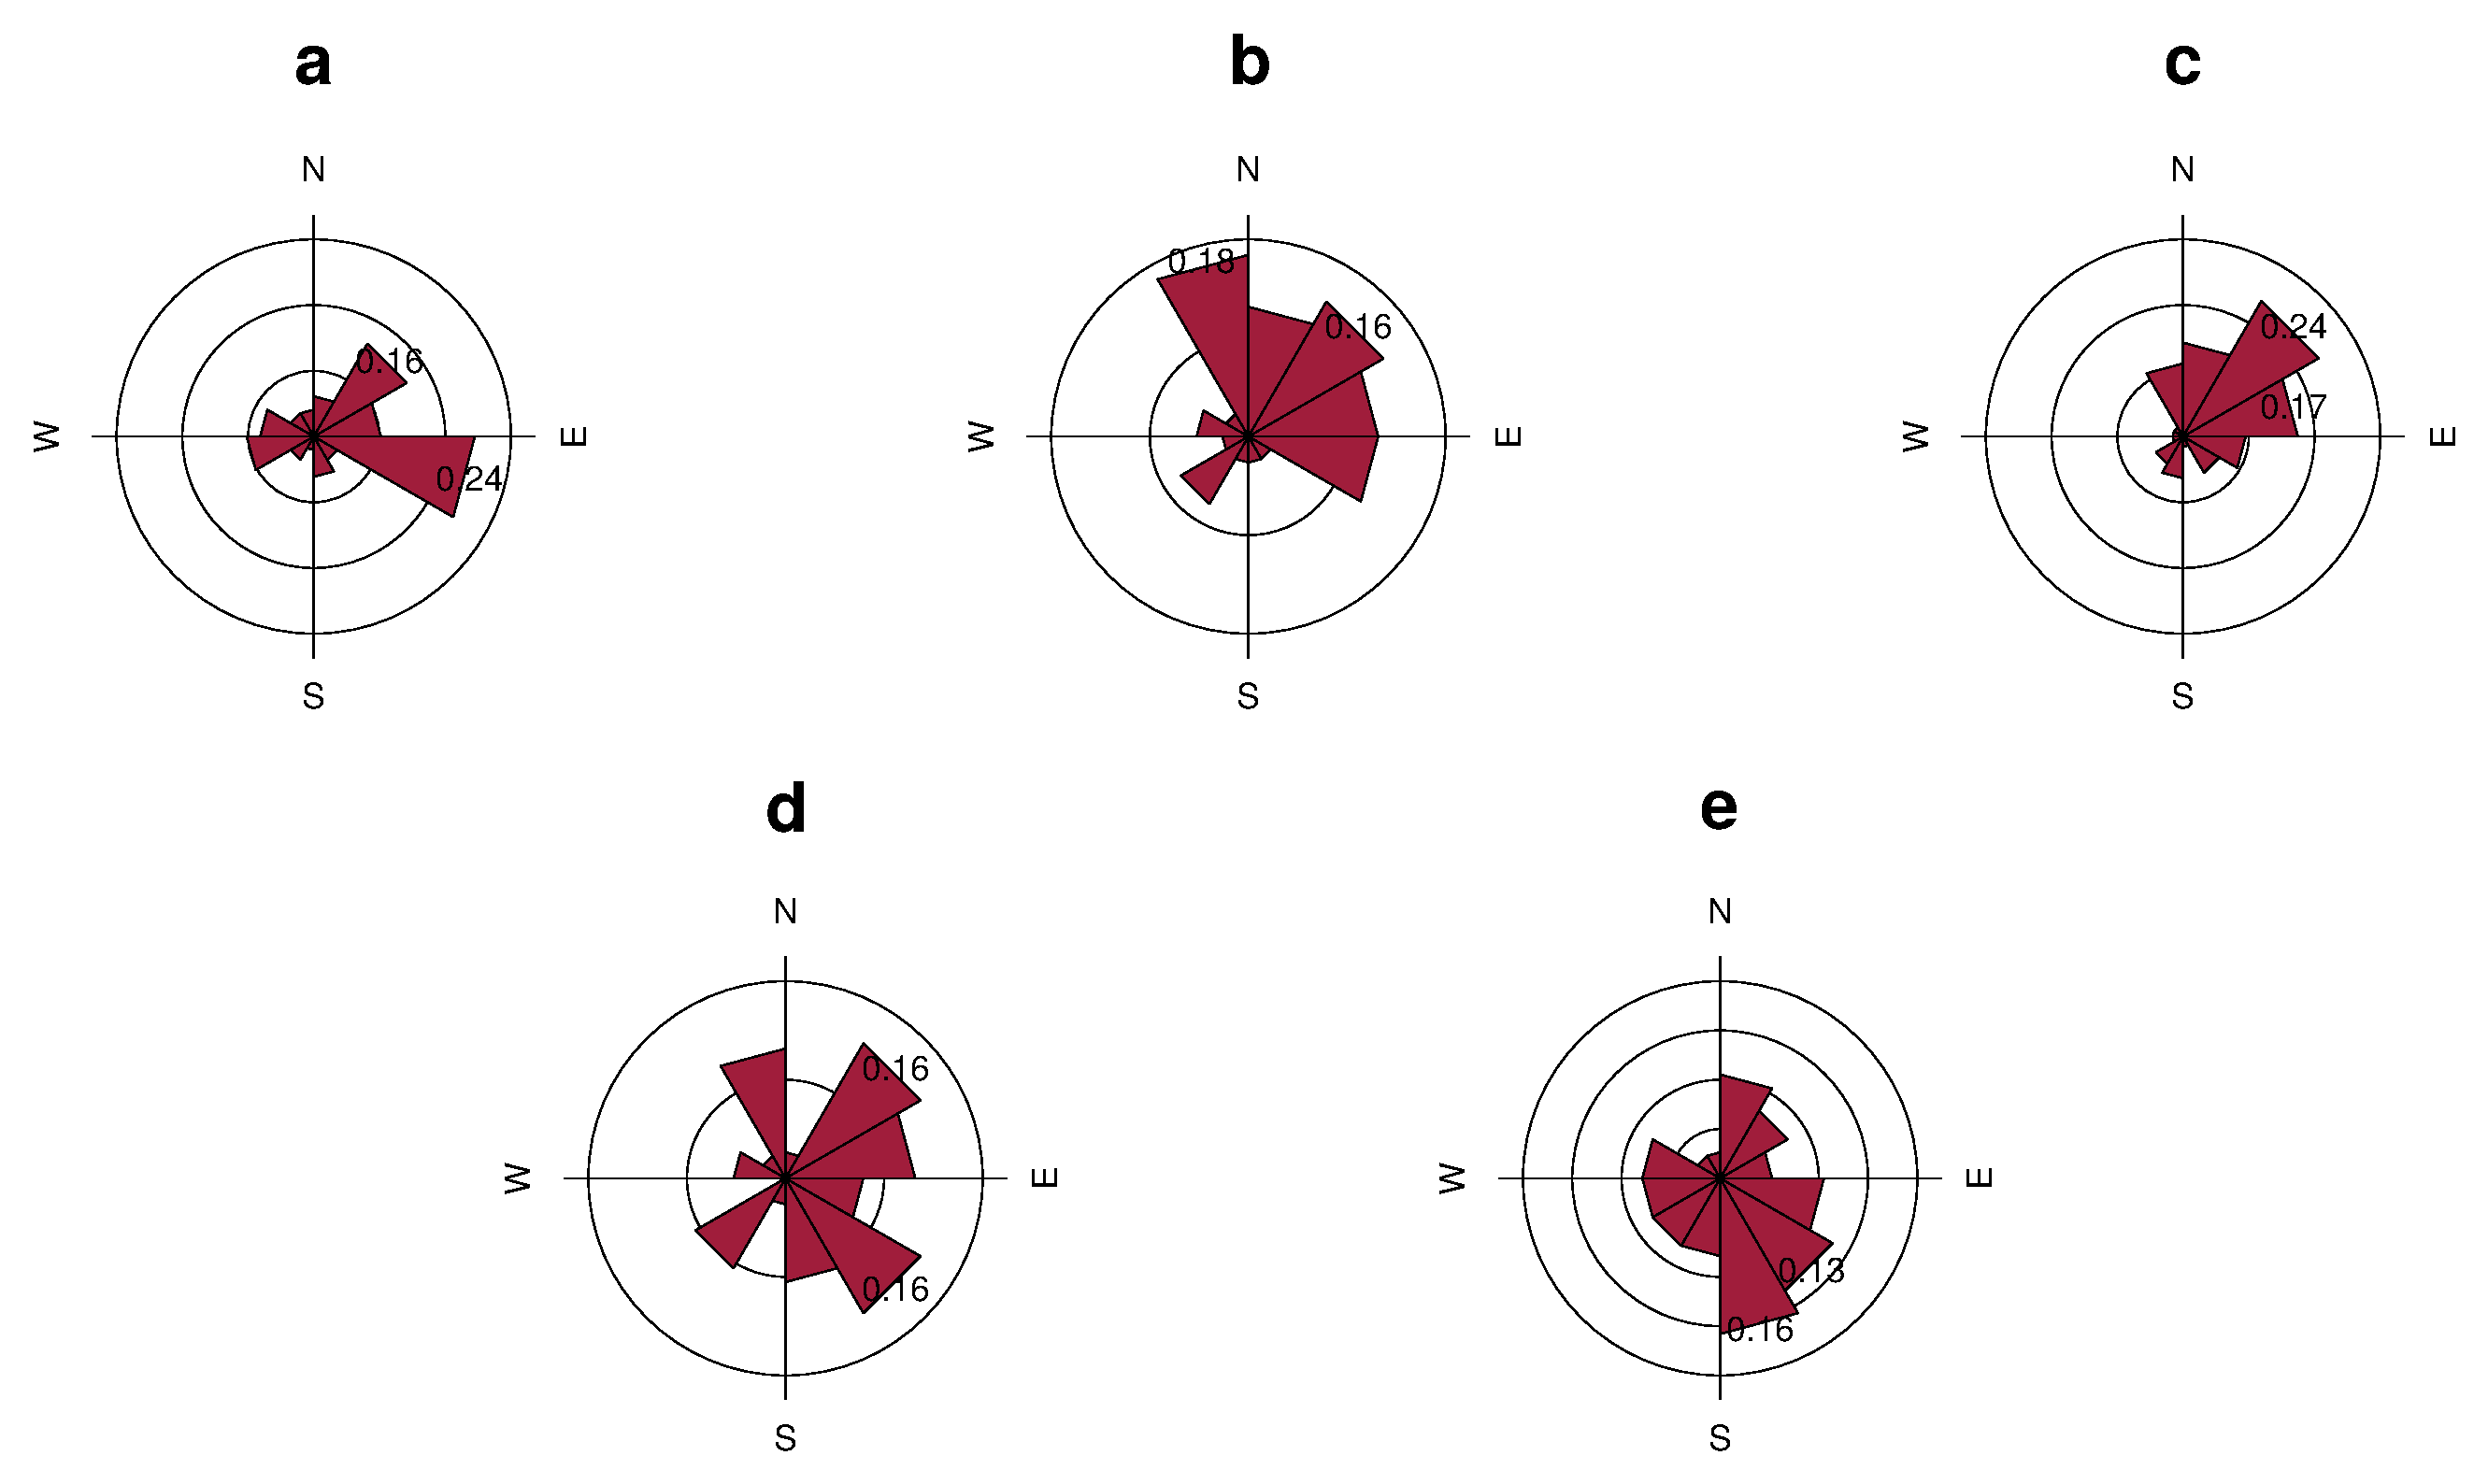
\includegraphics[width=1\textwidth]{../manuscript/artwork/Fig6.pdf}
  \caption{Rose diagrams showing the bearing patterns of samples from UA3c (a), UA4 (b), the elephant carcass (c) and UB4c (d: clock method, e: compass method).}
  \label{fig:6}
\end{figure*}

\begin{table*}[]
  \caption{Value and $p-value$ of circular uniformity test statistics.}
  \label{tab:3}
  \resizebox{1\textwidth}{!}{
    \begin{tabular}{lllllllllll}
      \hline
      &                                       & \multicolumn{2}{l}{Rayleigh} & \multicolumn{2}{l}{Kuiper} & \multicolumn{2}{l}{Watson} & \multicolumn{2}{l}{Rao}\\
      \cline{3-10}
      Sample                    & mean dir.   & $\bar{R}$       & $p$        & $V_{n}$  & $p$             & $U^{2}$  & $p$             & $U$      & $p$          \\
      \hline
      UA3c                      & 77.17°      & 0.268           & 0.029      & 2.4698   & <0.01           & 0.2967   & <0.01           & 271.8367 & <0.001       \\
      UA4                       & 35.79°      & 0.386           & 0.003      & 2.5656   & <0.01           & 0.3437   & <0.01           & 246.3158 & <0.001       \\
      \emph{P. antiquus}        & 54.64°      & 0.489           & 2.775e-07  & 3.4811   & <0.01           & 0.906    & <0.01           & 291.4286 & <0.001       \\
      UB4c (clock)              & 91.66°      & 0.276           & 0.054      & 1.8963   & 0.01<$p$<0.025  & 0.1937   & 0.025<$p$<0.05  & 255.7895 & <0.001       \\
      UB4c (compass)            & 151.17°     & 0.243           & 0.106      & 1.3944   & >0.15           & 0.1268   & >0.10           & 128.5263 & >0.10        \\
      \hline
    \end{tabular}
  }
\end{table*}

Table~\ref{tab:3} summarises the results of the circular uniformity tests. With regard to the UA3c sample, the Rayleigh test ($p-value=0.03$) rejected the null hypothesis of circular uniformity. The mean resultant length ($\bar{R}=0.27$) and the mean direction of 77° are thus significant, assuming the distribution is unimodal. However, the rose diagram (Fig.~\ref{fig:6}a) showed a bimodal distribution. The Kuiper, Watson and Rao omnibus tests, more powerful than the Rayleigh test in detecting multimodal deviation from uniformity, also rejected the null hypothesis of uniformity, therefore suggesting significant anisotropy in the distribution. For the UA4 sample and the subset of elephant bones, all the uniformity tests agreed in rejecting the null hypothesis in favour of a preferentially oriented distribution. The elephant sample, with respect to the other, showed significantly higher test results, thus stronger anisotropy. As suggested by the rose diagrams (Fig.~\ref{fig:6}c), this sample has a mean direction towards the NE (55°) and relatively low circular variance (29°).

The UB4c sub-samples had discordant test results when considering the omnibus statistics. However, according to the Rayleigh test, the mean resultant lengths ($\bar{R}$) and the mean directions were not significant for both sub-samples of measurements: $p-values>0.05$ failed to reject the null hypothesis of isotropy with 95\% confidence interval. This result is well confirmed by the Kuiper, Watson and Rao tests for the sub-sample of measurements recorded using the compass. Conversely, the omnibus tests failed to reject the hypothesis of uniformity for the other sub-sample of measurements recorded with the clock method. The rose diagram (Fig.~\ref{fig:6}d) suggested for the latter distribution strong multimodality, with uniformly spread peaks. The contrasting results obtained for the UB4c sub-samples are most probably due to the shape of those distributions. Indeed, the clock system, being less accurate, tends to produce a less dense distribution, more subject to show a multimodal shape when the distribution is actually uniform.

%% Woodcock diagram
The Woodcock eigenvalues ratio graph (Fig.~\ref{fig:7}a) presents the shape ($K$) and strength ($C$) of the distributions. Fig.~\ref{fig:7}b plots confidence levels of Monte-Carlo critical $C$ values, varying for sample sizes. The two sub-samples from Area B nearly overlapped, thus suggesting reliability of the orientation measurements collected using the clock system, although of low accuracy. The two sub-samples, together with the UA3c sample, having low $C$ values, plotted close to the origin of the ratio graph. Therefore, they indicate weak preferential orientation (UA3c) and significant randomness (UB4c). On the other hand, the UA4 and the elephant samples, with higher $C$ values, showed a stronger and significant tendency to orient preferentially. The shape parameter $K$ of the samples varied from $K=0.25$ for the UB4c sample measured with the compass, to $K=0.66$ for the one measured with the clock, to $K=0.48$ for the elephant sample. Overall, all the samples, except the UA3c one ($K=1.63$), plotted below the average shape value ($K=1$) between girdles and clusters distributions.

\begin{figure*}[]
  \centering
  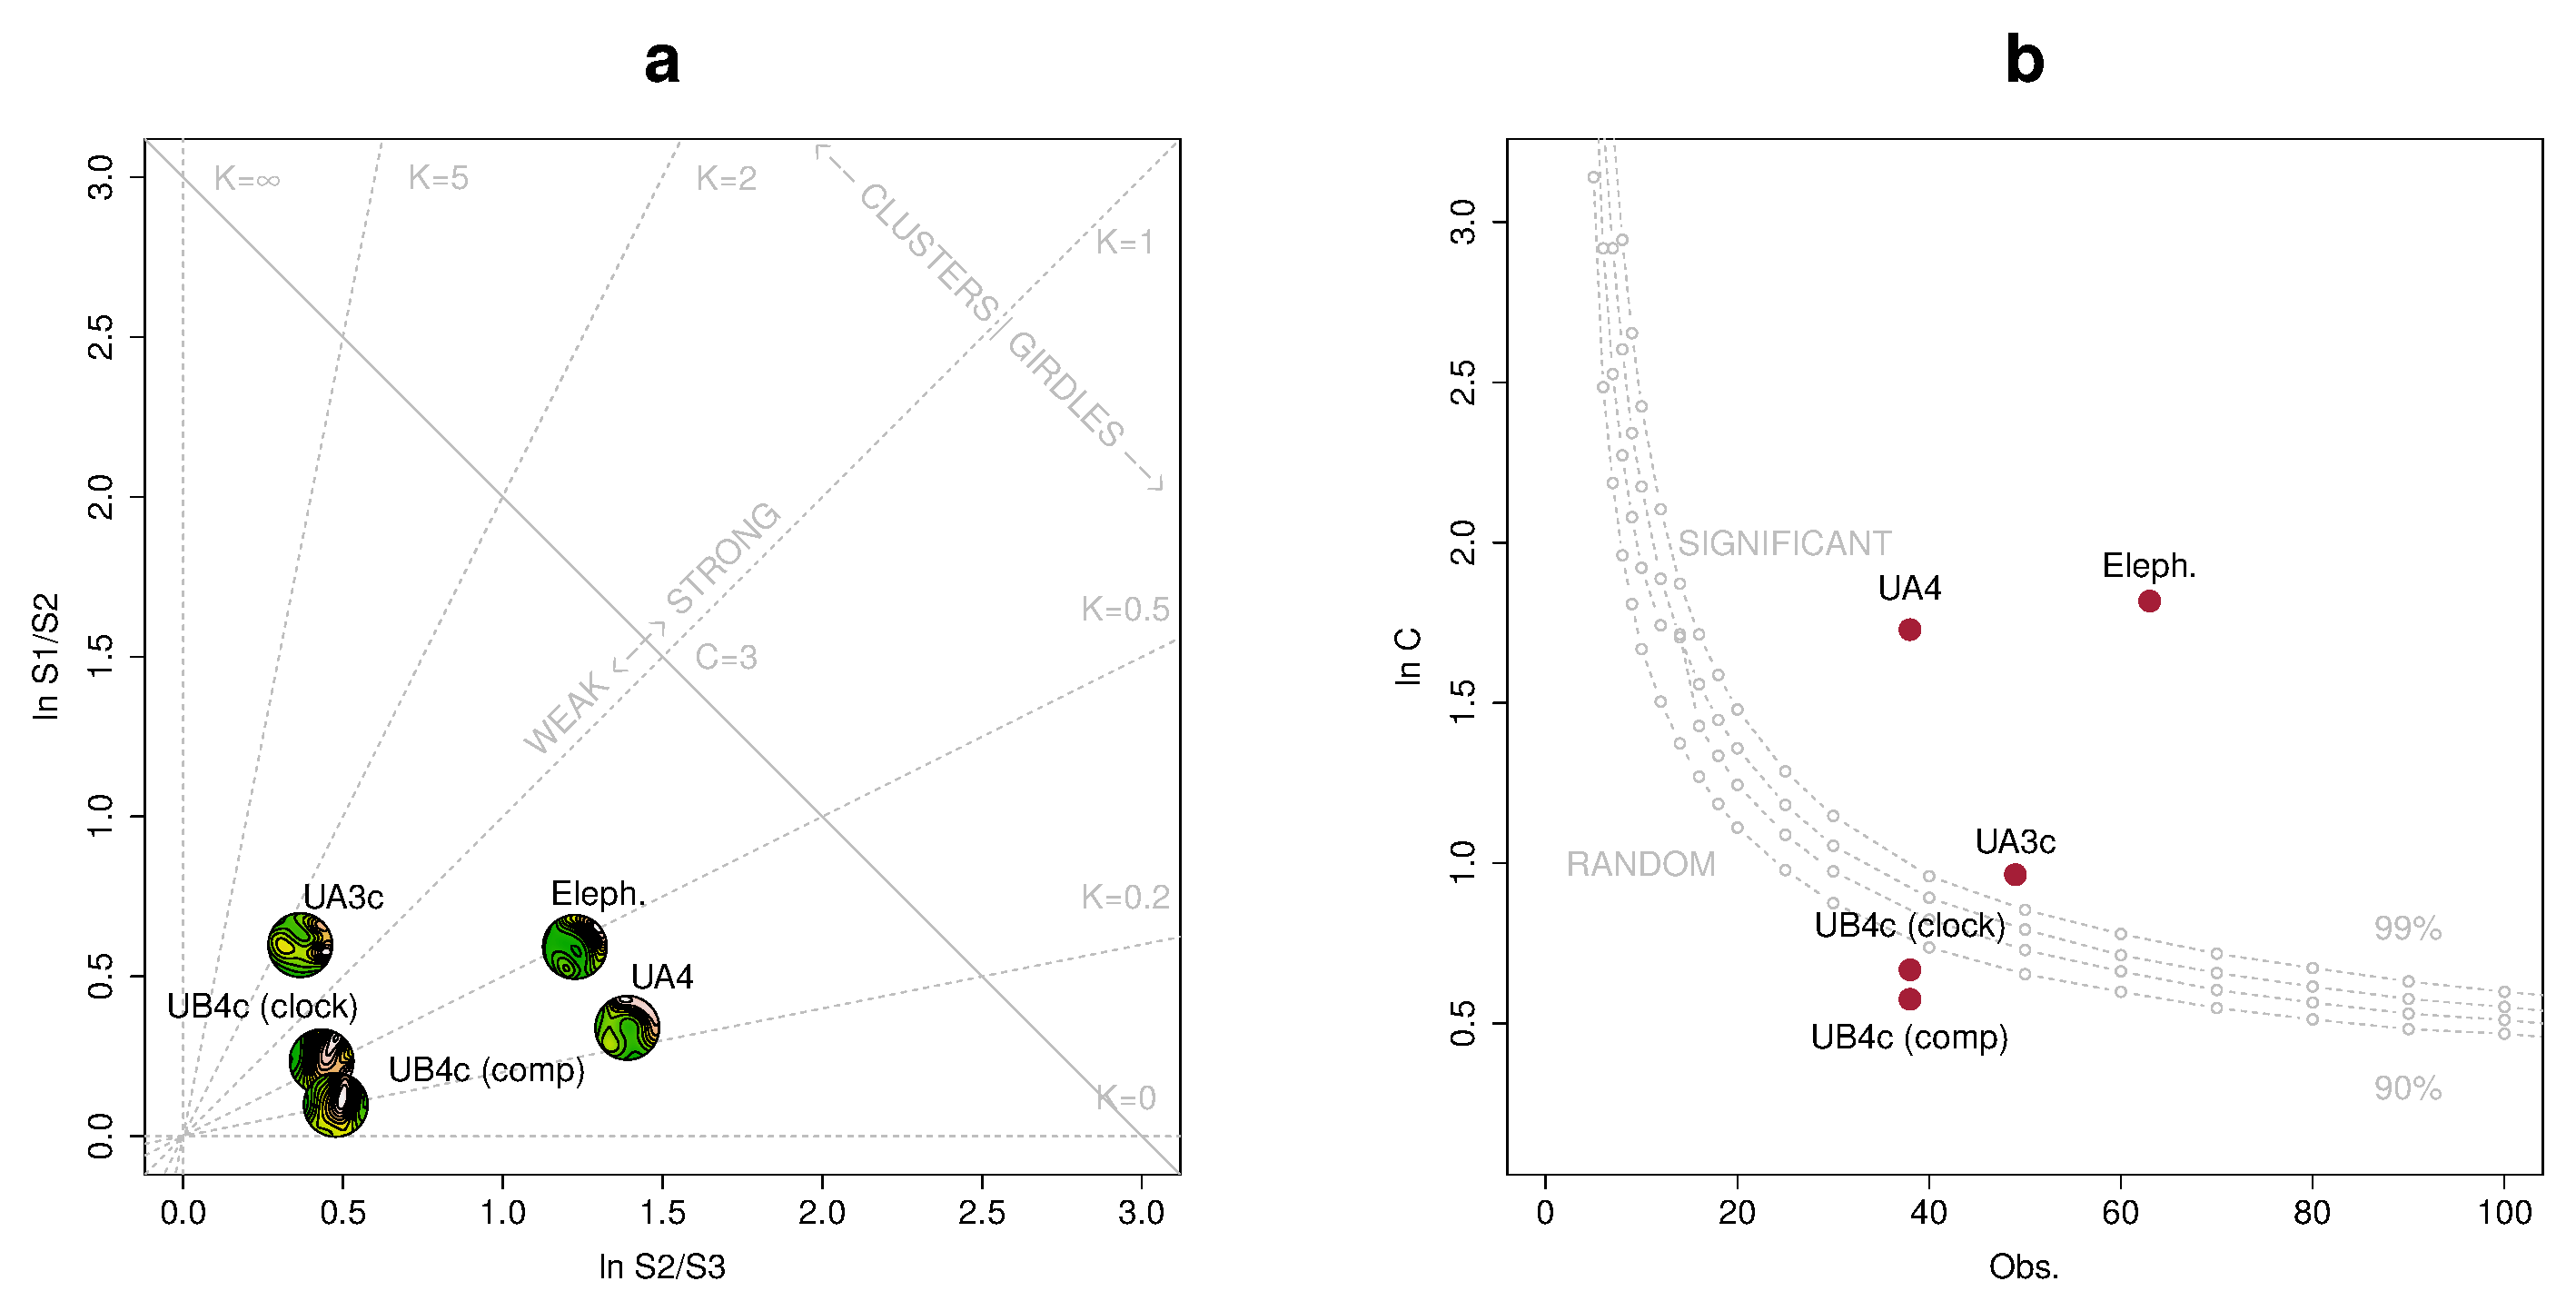
\includegraphics[width=1\textwidth]{../manuscript/artwork/Fig7.pdf}
  \caption{Woodcock's eigenvalues ratio graph (a) and plot of the Monte-Carlo critical $S_1/S_3$ test values, for varying sample sizes and confidence levels (b), modified from \cite{Woodcock1983}.}
  \label{fig:7}
\end{figure*}

%% Benn diagram
The Benn diagram (Fig.~\ref{fig:8}) resembles the Woodcock ratio graph (Fig.~\ref{fig:7}a). The samples from units UB4c and UA3c clearly plotted at a distance from the UA4 and the elephant samples. The UB4c samples plotted in the upper corner of the ternary graph, with the UB4c sub-sample of measurements taken with the compass exhibiting more isotropy. The UA3c sample, with an elongation index similar to the elephant sample, but higher isotropic index, plotted towards the centre. Compared to the ranges of fabrics recorded for modern natural processes (debris flow and runoff), the fabric from the UA3c and UB4c units plotted well inside the cluster of debris flows, with the UB4c (comp) sample suggesting even more random orientations. On the other hand, the sample of elephant remains, which lie mostly on UA4 and are covered by UA3c, plotted significantly close to the sample from unit UA4. They both presented the lowest isotropy index ($IS$), but not high elongation index ($EL$). Thus, they plotted in the average between linear and planar orientations, at the margins of the range of runoff processes. Yet they still plotted within the cluster of debris flows fabrics. Moreover, as suggested also by the uniformity tests (Tab.~\ref{tab:3}), the elephant sample showed a more linear attitude with respect to the UA4 sample.

\begin{figure*}[]
  \centering
  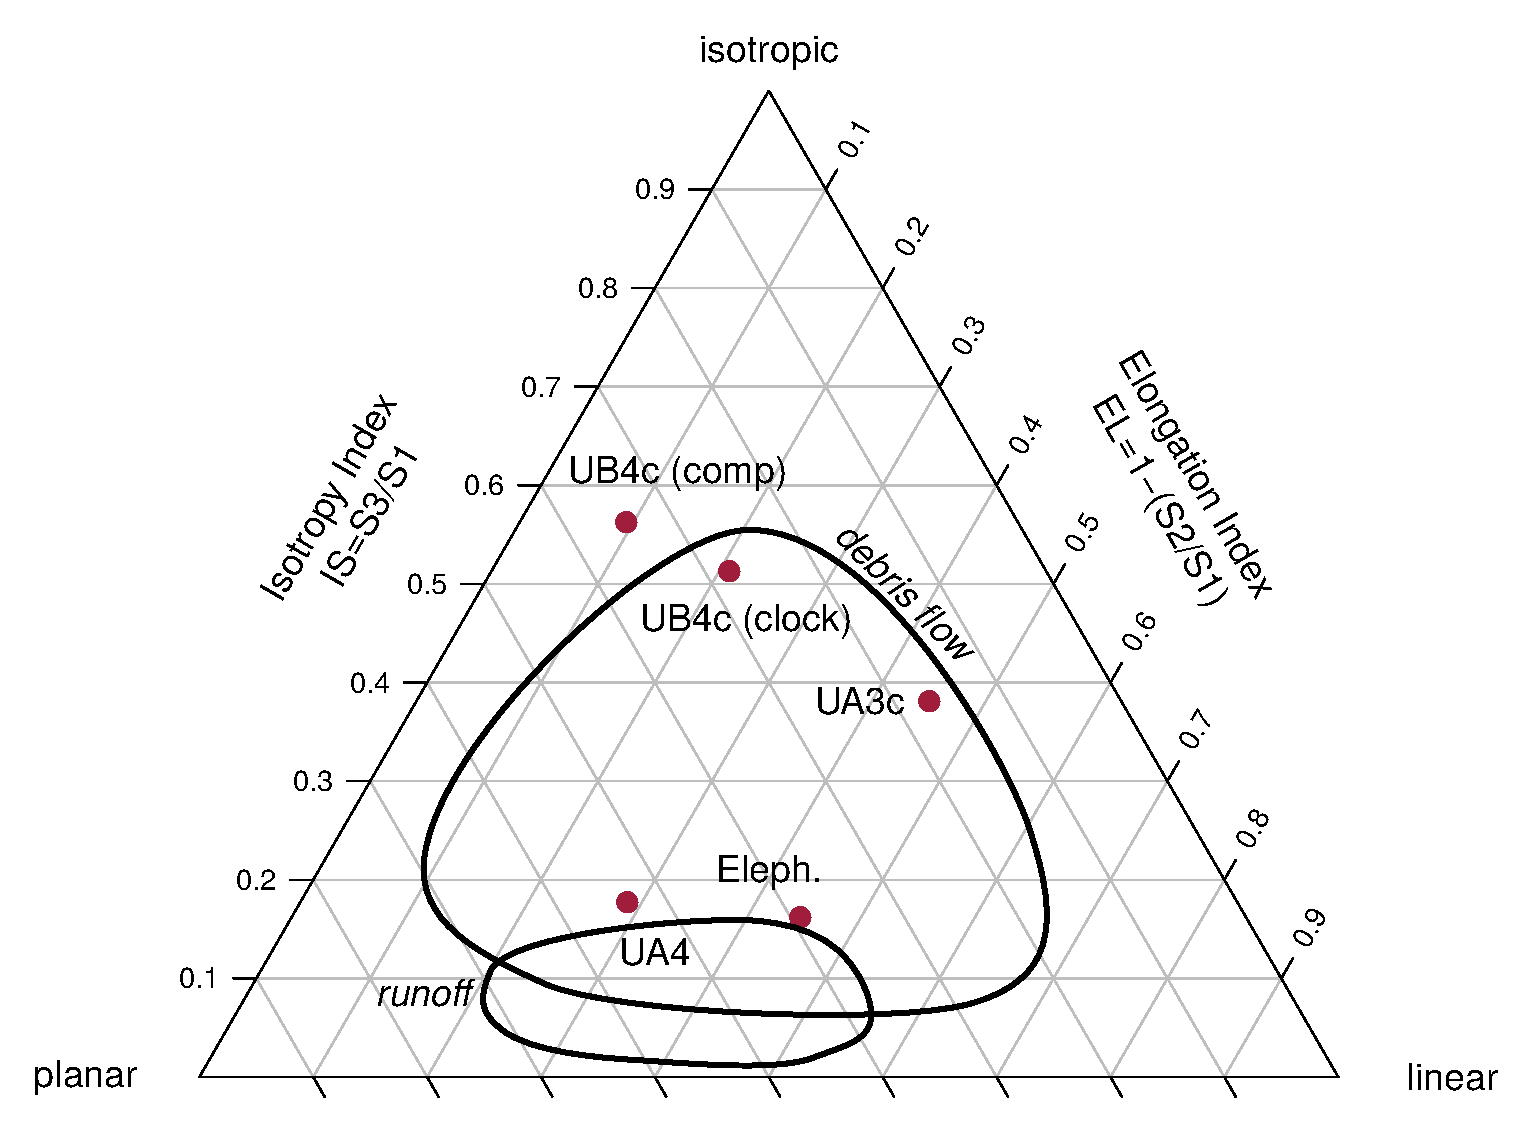
\includegraphics[width=.5\textwidth]{../manuscript/artwork/Fig8.pdf}
  \caption{Benn's diagram. Fabric ranges of natural processes modified from \cite{Lenoble2004}.}
  \label{fig:8}
\end{figure*}

\subsection{Vertical distribution}

%% UA3c/4c
Fig.~\ref{fig:9} compares the vertical distribution of the finds from units UA3c and UA4, by means of empirical density functions of the minimum distances (d) from each specimen to the UA3c/4 erosional contact (Fig.~\ref{fig:5}a). Three lithic artefacts (two flakes and one tool) from the UA3c unit, not included in Fig.~\ref{fig:9}, plotted within 15~cm from the interpolated surface. Only one flake has been found in the lower UA4, at about 17~cm from the UA3c/4 contact, together with three chips. Despite the scarcity of debitage products in this area, waste products (debris/chip) are relatively well represented (16\% of the UA3c sample). Their vertical dispersion approximated a normal distribution ($\mu=0.24$, $\sigma=0.15$): the Kolmogorov-Smirnov and Shapiro tests failed to rejected the null hypothesis of normality ($p-value$=0.83 and 0.075, respectively). Notably, the distributions of the faunal remains from the same unit UA3c were all right skewed, with means ($\mu$) about 20~cm above the UA3c/4 contact. Nevertheless, the Welch two sample t-test ($p-value=0.61$) failed to reject the null hypothesis that the lithic and faunal sample means are equal. The total distribution of remains from unit UA3c showed a unimodal distribution, skewed to the right, with mode in the proximity of the UA3c/4 surface. Similarly, the vertical distribution of faunal remains recovered from unit UA4 concentrate in the first 10~cm below surface. The density functions altogether clearly confirmed one of the main observations assessed during excavation, namely that, with the elephant remains lying at the UA3c/4 contact and covered by unit UA3c, most of the faunal and lithic material were recovered from unit UA3c (Fig.~\ref{fig:2}) and predominantly in the proximity of the UA3c/4 contact (Fig.~\ref{fig:9}).

\begin{figure*}[]
  \centering
  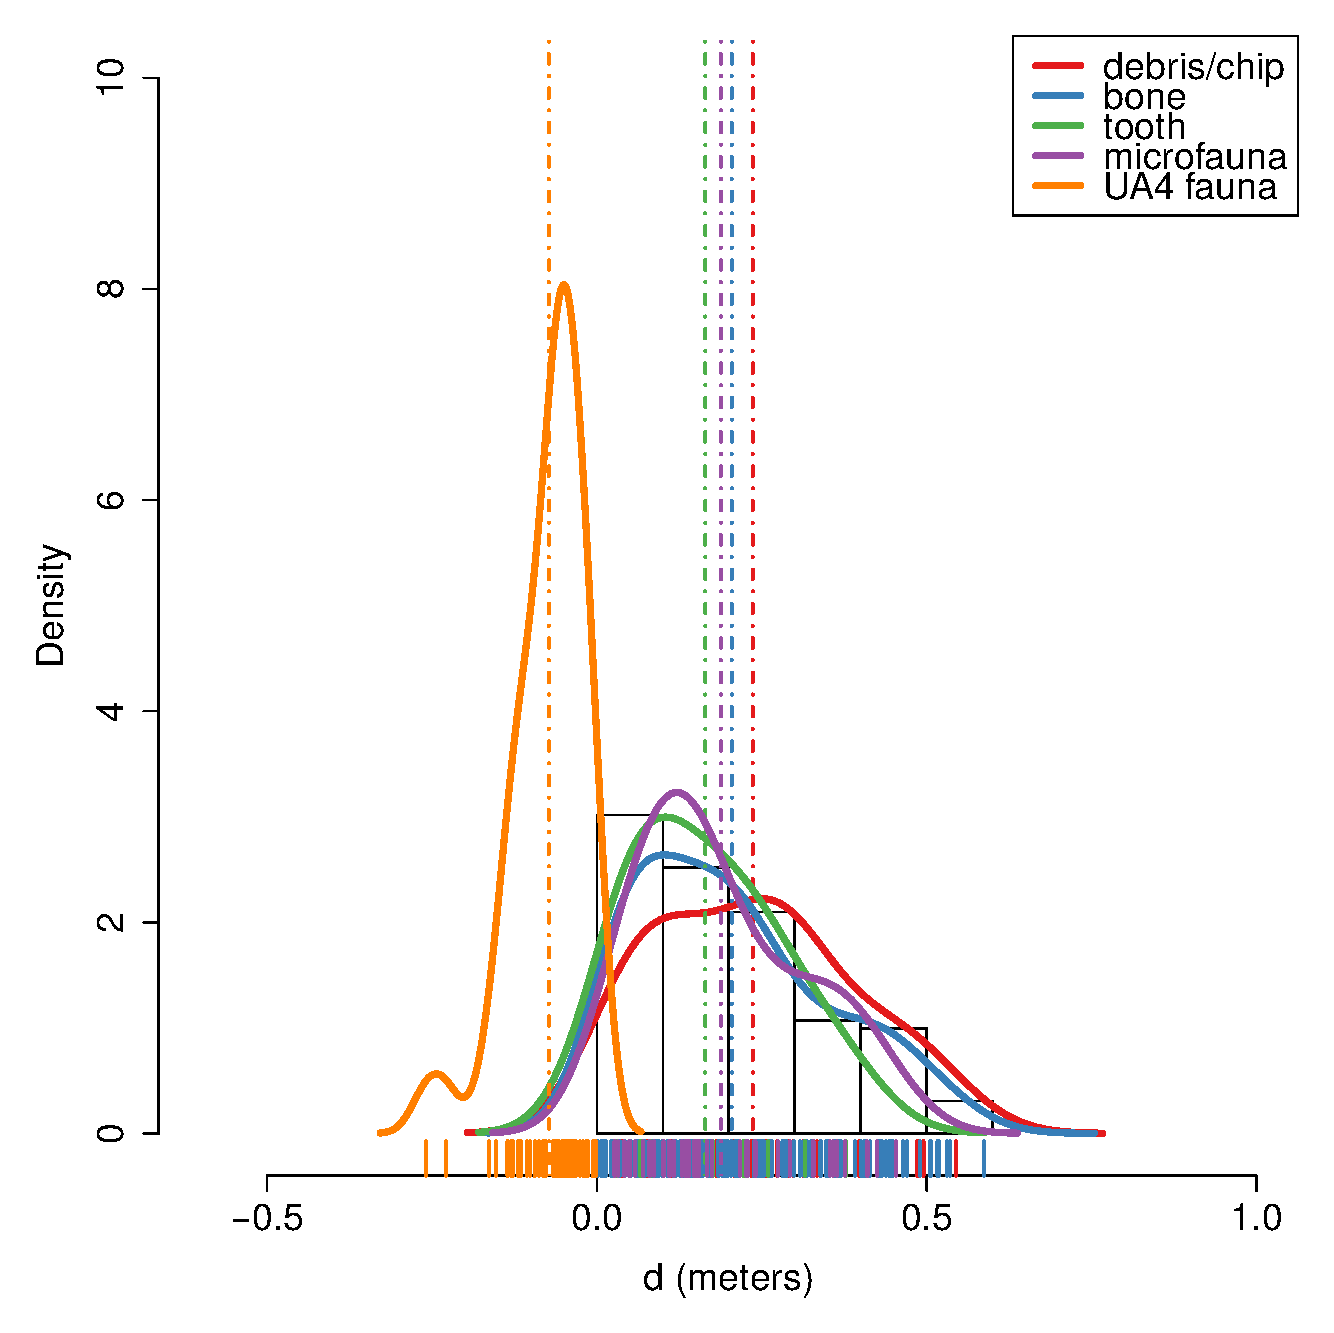
\includegraphics[width=.5\textwidth]{../manuscript/artwork/Fig9.pdf}
  \caption{Empirical density functions of minimum orthogonal distances (d) to the UA3c/4 surface. The histogram represents the total distribution of remains from UA3c; dashed lines indicate mean values.}
  \label{fig:9}
\end{figure*}

%% UB5a
Fig.~\ref{fig:10} shows the empirical density functions of the minimum distances from each specimen from Area B to the UB4c/5a erosional contact (Fig.~\ref{fig:5}b). The combined distribution of any type of find from the UB5a unit (Fig.~\ref{fig:10}a) skewed to the left with a short tail (up to -0.3~m). The mode, between 5 and 10~cm below the roof of UB5a, indicates a general concentration of material very close to the contact of this unit with the overlying UB4c, in accordance with the mean distribution of the different classes of remains. Although the majority of both the lithic and faunal assemblages were found in the uppermost 15~cm of UB5a, few debris/chips and bone fragments occur lower in the sequence, yet no more than 30~cm below the roof of this unit. Very few flakes, three tools and no cores have been found in this unit. As a whole, the lithic assemblage from UB5a, mostly composed by debris/chips, is only 7\% of the most conspicuous assemblage from UB4c.

%% UB4c
The global distribution of unit UB4c was right skewed (up to almost 0.6~m) and centred at about 5~cm above the contact with the underlying unit UB5a (Fig.~\ref{fig:10}b). Almost 30\% of the sample fell exactly at the erosional contact that separates UB4c from UB5a. The density estimations of the lithic debris/chip, flakes, tools and faunal remains significantly overlap, whereas the distribution of the six cores shows a bimodal shape with peaks at 5 and 20~cm above the contact. Moreover, the Welch Two Sample t-test of the lithic and faunal sample means failed to reject the null hypothesis ($p-value=0.6295$).

\begin{figure*}[]
  \centering
  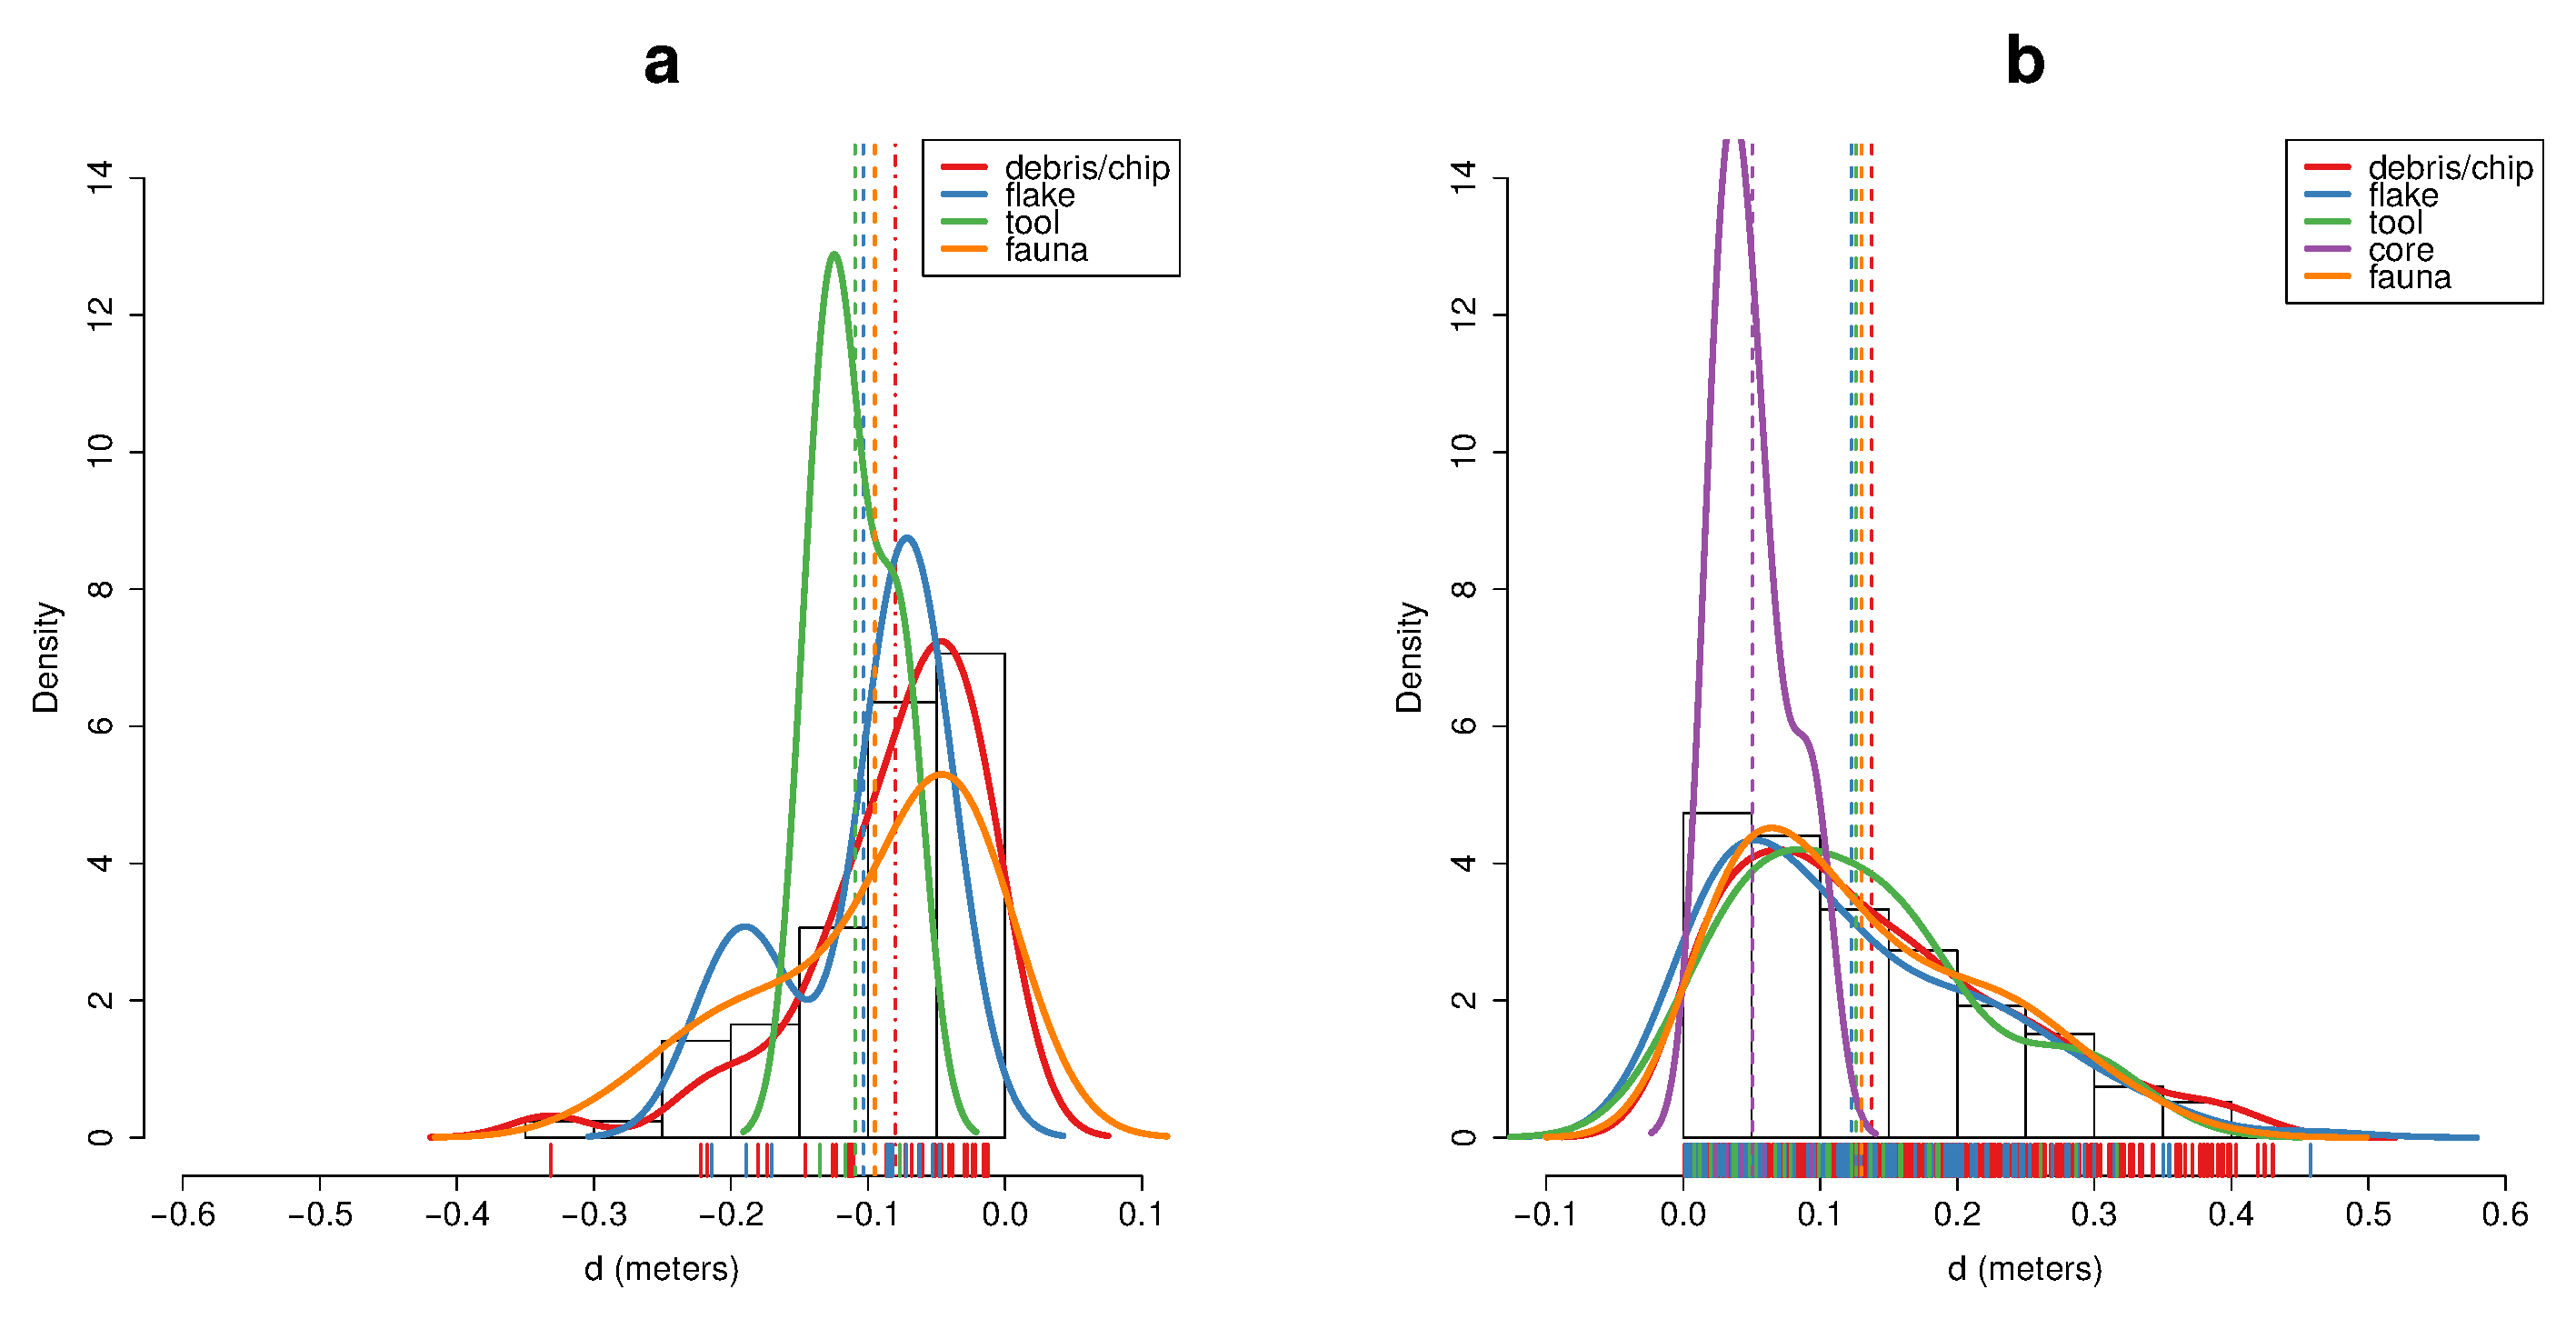
\includegraphics[width=1\textwidth]{../manuscript/artwork/Fig10.pdf}
  \caption{Empirical density functions of minimum orthogonal distances (d) to the UB4c/5a surface. The histogram represents the total distribution of remains from UB5a (a) and UB4c (b); dashed lines indicate mean values.}
  \label{fig:10}
\end{figure*}

\subsection{Point pattern analysis}

%\subsubsection{Area A}
Results of the point pattern analysis are complementary to those obtained from the analysis of the fabric and vertical distributions. Regarding Area A, kernel density estimation and three-dimensional functions were applied in order to quantitatively depict the spatial distribution of the lithic assemblage in relation to the elephant skeleton. Fig.~\ref{fig:11}a shows the smoothing kernel intensity estimation of the faunal assemblage from the UA3c unit. Contour lines delimit the density of the lithic sample. The partial skeleton of the \emph{P. antiquus} is superimposed on it. A preliminary visual examination of the plot suggests a homogeneous distribution of lithics (mostly debris/chips) and fossils. Spots of higher density appear to be spread around and in association with the elephant remains.

The univariate pair correlation function of the joined lithic assemblage from the UA3c and UA4 units (Fig.~\ref{fig:11}b) suggests aggregation of finds. The estimated $\hat{g}_3(r)$ function (black solid line) wanders above the benchmark value (red dotted line) until values of $r=0.8$. However, for distances between 35 and 65~cm, it lies above the grey envelope of significance for the null hypothesis of CSR, indicating that at those distances artefacts occur significantly closer than expected in the case of random processes. For values of $r>0.8$, the function stabilises at values close to 0, suggesting a Poisson distribution. The plot illustrates the random distribution of finds between patches of clusters that we observe in Fig.~\ref{fig:11}a.

The histogram in Fig.~\ref{fig:11}c shows the density of the distances calculated from each artefact to the nearest-neighbour elephant remain. A right skewed distribution, with a prevalent peak at 10~cm and mean ($\mu$) 30~cm is an indication of the relatively strong aggregation of lithics around the mass of the elephant skeleton.

\begin{figure*}[]
  \centering
  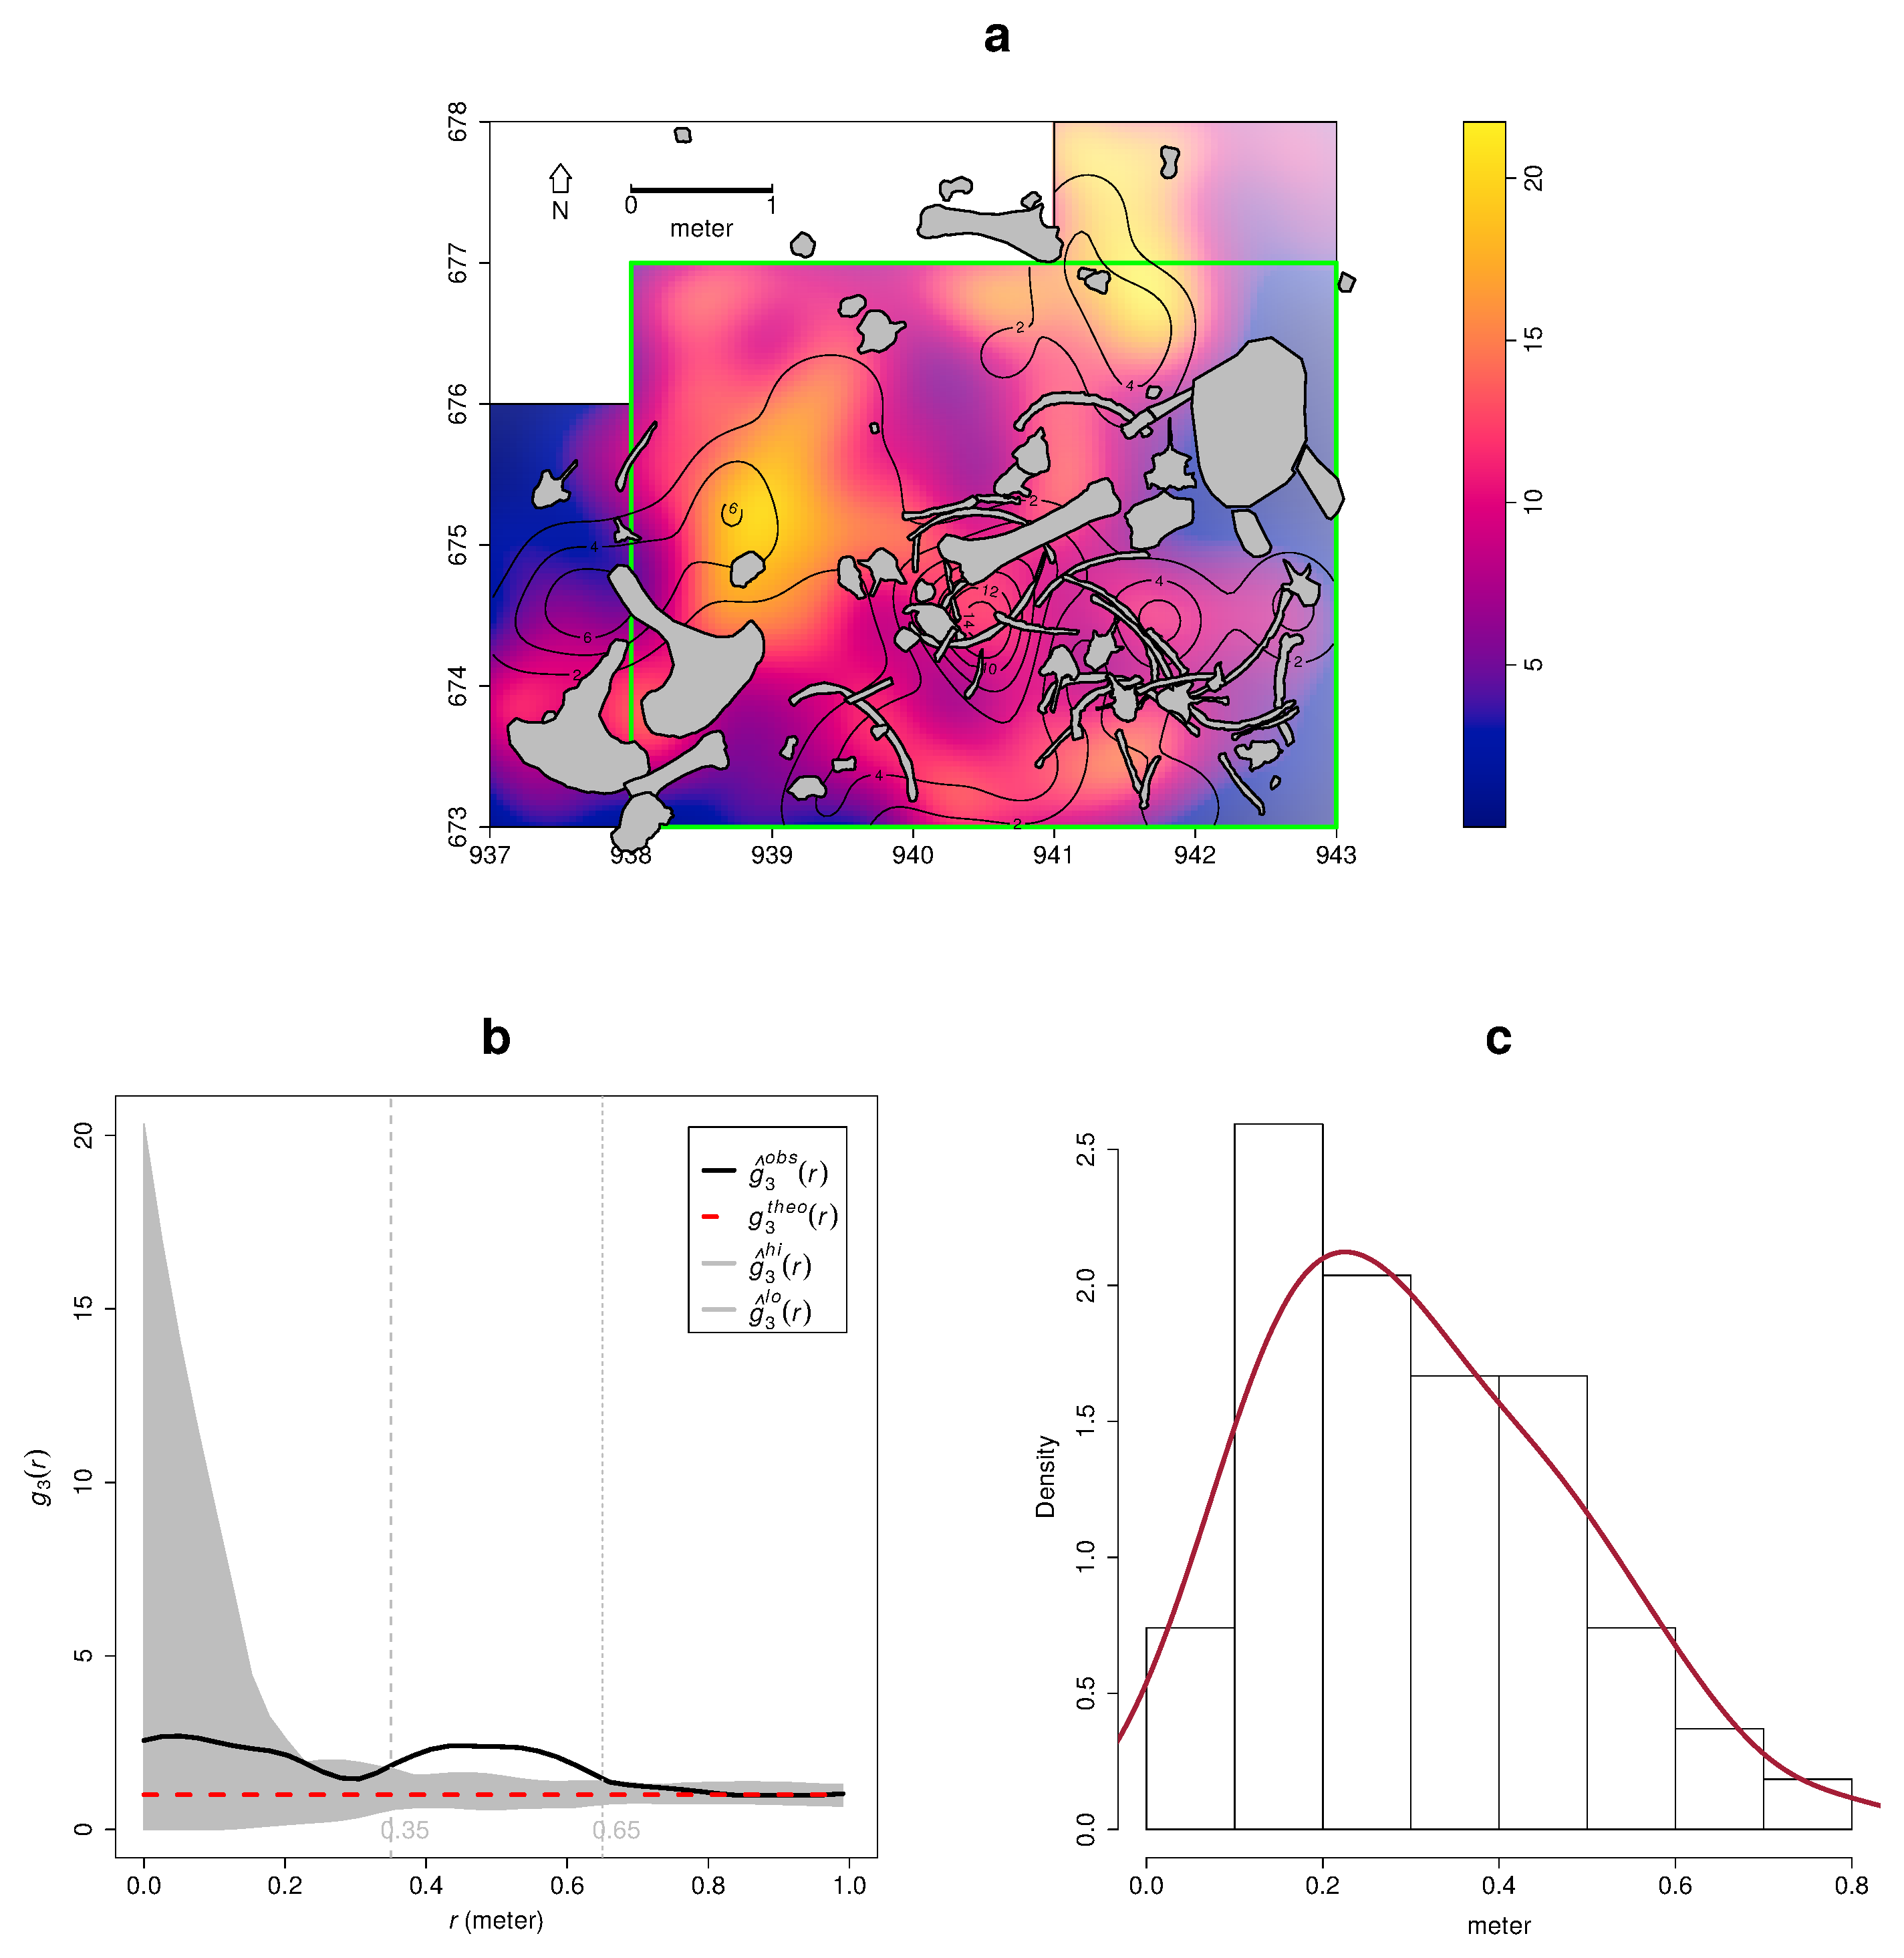
\includegraphics[width=1\textwidth]{../manuscript/artwork/Fig11.pdf}
  \caption{Kernel smoothed intensity function of the faunal assemblages from UA3c. Isolines mark the density of the lithic artefacts from UA3c (a). Pair correlation function ($g_3(r)$) of a three-dimensional pattern of lithic artefacts from UA3c and UA4. Grey envelope of 999 Monte Carlo simulations under the CSR null hypothesis (b). Three-dimensional distance from each lithic artefact from UA3c and UA4 to the nearest neighbour elephant remain (c).}
  \label{fig:11}
\end{figure*}

%\subsubsection{Area B}

As for Area B, the analysis focused on the spatial distribution and cross-correlation of the assemblages from UB4c and UB5a. Figs.~\ref{fig:12}a,b respectively show kernel density estimations of the combined lithic and faunal assemblages from both the units analysed. Despite the samples size difference, a first visual examination suggests the presence of interesting spatial structures. Regarding the UB4c unit (Fig.~\ref{fig:12}a), the high density of material concentrated around the western square 934/600 suggests that the pattern could have been the result of an inhomogeneous, non-uniform depositional process. Visual comparison of the density plot with the elevation model of the erosional contact between the UB4c and UB5a units (Fig.~\ref{fig:5}b) suggests positive correlation between lower elevations (topographic depressions) and higher density of remains.

Fig.~\ref{fig:12}c shows the results of the $\rho$-function, which estimates the intensity of the UB4c sample assemblage as a function of the covariate underlying topography created by the erosional event. Within the range of elevation between 350.2 and 350.4~m, the occurrence of finds is higher and the intensity decreases with the rise of elevation, i.e., finds are more likely to be found at lower elevations than would be expected if the intensity was constant. Spatial Kolmogorov-Smirnov (KS) and Berman's $Z_2$ \citep{Berman1986} statistics were used in order to test the dependence of the UB4c pattern on the covariate erosional surface. Both KS ($D=0.11952$, $p-value=7.772e-16$) and $Z_2$ ($Z2=-7.8447$, $p-value=4.34e-15$) significantly rejected the null hypothesis of CSR. Although the tests suggested evidence that the intensity depends on the covariate, the effect of the covariate is weak and it seems to have no discriminatory power. The ROC curve and AUC statistics (0.56), which measure the strength of the covariate effect, suggest that the underlying UB4c/5a topography does not completely explain the localised high density of occurrence in the UB4c.

Relative spatial segregation seems to occur between the assemblages from UB4c (Fig.~\ref{fig:12}a) and UB5a (Fig.~\ref{fig:12}b), with high density of the former distribution corresponding to low density of the latter. The former analysis of the vertical distribution showed that the two assemblages occur very close to their stratigraphic contact (Fig.~\ref{fig:10}). In order to further investigate the spatial interaction between the two depositional events, we applied multitype pair correlation $g_{ij}(r)$ and nearest-neighbour $G_{ij}(r)$ functions. Fig.~\ref{fig:12}d shows the estimated values of the multivariate $\hat{g}_{ij}(r)$ function against the envelope of the null hypothesis, obtained by randomly shifting the position of remains from the two distributions in 199 Monte Carlo simulations. For fixed values of $r$ less than 30~cm the observed function lies below the benchmark value of independence, thus indicating segregation; but it wanders at the lower edge of the grey envelope. For fixed distances of $r>0.3$~m the observed and theoretical lines significantly overlap. Overall, the function suggests independence of the two point processes (UB4c and UB5a) at multiple scales. However, the estimated $\hat{G}_{ij}(r)$ function (Fig.~\ref{fig:12}e), running well below the significance grey envelope for fixed values of $r>0.3$~m, confirms that the nearest-neighbour distances between remains from UB4c and UB5a are significantly longer than expected in the case of independent processes. Interestingly, at values of $r<0.2$~m the observed function failed to reject the null hypothesis of Complete Spatial Randomness and Independence (CSRI).

\begin{figure*}[]
  \centering
  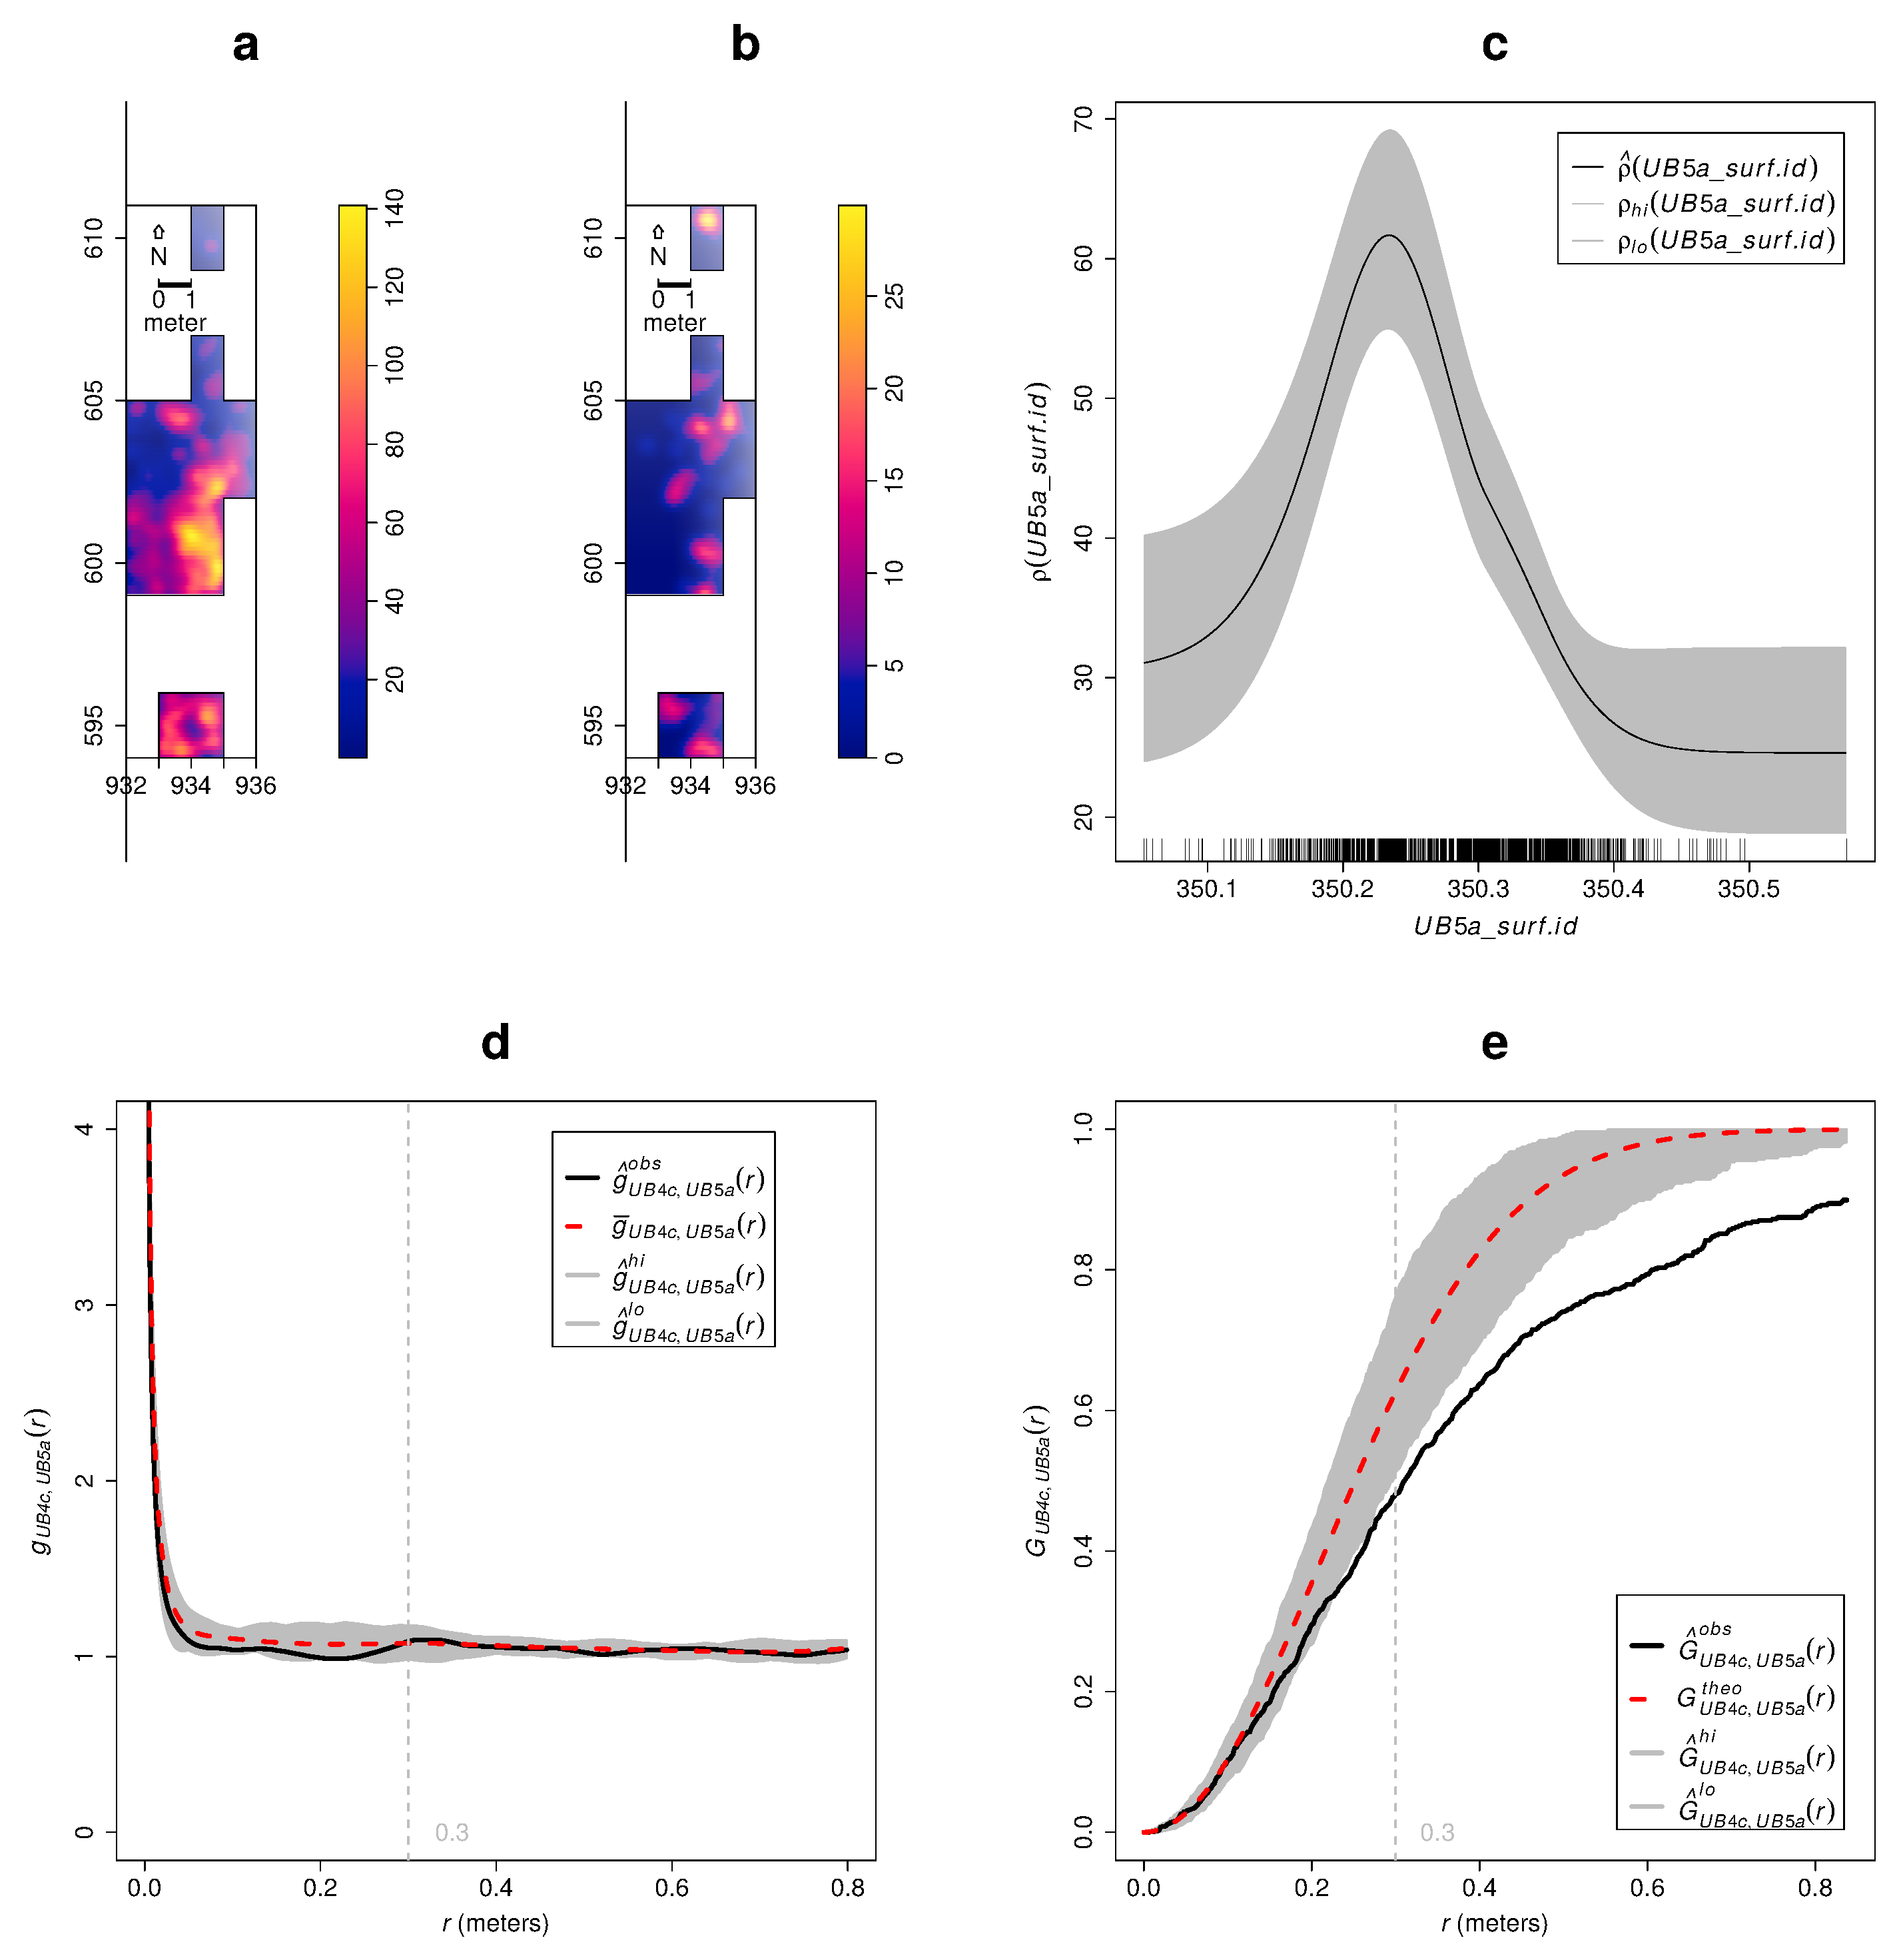
\includegraphics[width=1\textwidth]{../manuscript/artwork/Fig12.pdf}
  \caption{Kernel smoothed intensity function of the lithic and faunal assemblages from UB4c (a) and UB5a (b). Smoothing estimate of the intensity of remains from UB4c, as a function of the erosional surface UB4c/5a. Grey shading is point-wise 95\% confidence bands (c). Cross-pattern pair correlation function ($g_{ij}(r)$) between the UB4c and UB5a distributions. Grey envelope of 199 Monte Carlo simulations under the independence of components null hypothesis (d). Multitype nearest-neighbour function ($G_{ij}(r)$) between the UB4c and UB5a distributions (e).}
  \label{fig:12}
\end{figure*}

\section{Discussion}

%% Intro
Recent excavations at the Middle Pleistocene site of Marathousa~1 have unearthed in one of the two investigated areas (Area A) a partial skeleton of a single individual of \emph{Palaeoloxodon antiquus}, whose bones are in close anatomical association, and spatially and stratigraphically associated with lithic artefacts and other faunal remains. In Area B, 60~m to the South of Area A, we collected a much higher number of lithic artefacts \citep{Tourloukis}, spatially and stratigraphically associated with other faunal remains, including isolated elephant bones, cervids and carnivores among others \citep{Konidaris}. The two areas are stratigraphically correlated, the main fossiliferous layers (UA3c and UB4c) representing a massive depositional process, such as a hyperconcentrated flow that dumped material in a lake margin context \citep{Karkanas}. To date, evidence of butchering (cut-marks) has been identified on two bones of the elephant skeleton from Area A, as well on elephant and other mammal bones from Area B \citep{Konidaris}.

However, due to the secondary depositional nature of the main fossiliferous horizon, it is of primary importance to evaluate the degree and reliability of the spatial association of the lithic artefacts with the faunal remains, and especially with the elephant skeleton. In order to tackle our main objective, we applied a comprehensive set of spatial statistics to the distributions of the archaeological and zooarchaeological/palaeontological remains from relevant stratigraphic units of the two areas of investigation. Preliminary results of our analyses are here discussed for both areas.

\subsection{Fabric analysis}

%\subsubsection{UA3c/UA4c}
The analysis of the orientation (plunge and bearing) of subsets of remains, mostly bone, wood fragments and lithic artefacts, showed different patterns for the two main find-bearing units. In Area B, two sub-samples from the same stratigraphic unit were analysed, in order to asses the reliability of the orientation data measured with the clock system. Due to the different shapes of the distributions (Figs.~\ref{fig:6}d,e), test statistics reported contrasting results (Tab.~\ref{tab:3}). Indeed, the clock system, recording non-continuous circular data, tends to produce a distribution more subject to show a multimodal shape when it is actually uniform. However, the two sub-samples nearly overlapped when plotted in the three-dimensional Woodcock (Fig.~\ref{fig:7}) and Benn (Fig.~\ref{fig:8}) diagrams, thus suggesting some degree of reliability of the clock method. Nevertheless, despite minor differences between the two samples, caution should be paid in analysing grouped circular data.

%\subsubsection{UA4}

The test results (Tab.~\ref{tab:3}) for the UA4 sample and the sample of elephant remains - which lie on unit UA4 and are covered by UA3c - indicated significant preferential orientations towards the NE (Figs.~\ref{fig:6}b,c). As shown by the Woodcock's (Fig.~\ref{fig:7}) and the Benn's diagrams (Fig.~\ref{fig:8}), these samples plotted together at a distance from the others. Such convergence suggests that the elephant carcass, the other faunal remains and the organic material, deposited on unit UA4, were subject to the same processes. Far from the isotropic corner in the Benn's diagram these two samples from Area A plotted approximately in between the linear and planar extremes, with the elephant sample showing a more linear fabric. When the results published by \cite{Bertran1997} and \cite{Lenoble2004} from observations of fabrics in modern subaereal slope deposits were used as a reference, the two samples aggregated at the extreme margins of runoff processes. Yet, they plotted well within the cluster of debris flows and relatively distant from the linear corner.

Although \cite{Bertran1997} studied runoff deposits from different environments (channel-lag gravels in rills, small gullies, and inter-rill surfaces on alpine slopes; and faintly laminated gravel lenses on an inactive, small colluvial fan), this result is consistent with the exposure of unit UA4 to overland water-laden processes that occurred before the flood event UA3c/UB4c. Notably, the erosive nature of low-energy processes triggered by rain-water has been observed on lacustrine floodplains, and is associated with anisotropic patterns in autochthonous assemblages \citep{Cobo-Sanchez2014,Dominguez-Rodrigo2014,Garcia-Moreno2016}.

Pockets of thinly bedded organic-rich silty sands have been found mixed in UA4. These sands in Area A resemble the UB5b/c sandy deposit in Area B, which is associated with relatively high energy fluvial flows entering the lake margins \citep{Karkanas}. Eventually, such relatively high energy flood (UB5b/c) would have had the power to significantly reorient elements of the elephant carcass and slightly displace them. However, the elephant skeleton clearly lies on top of unit UA4 and is covered by UA3c (see Fig.\ref{fig:4}).

Moreover, unlike bones with a tubular shape (i.e., long bones), ribs and vertebrae are prone to orient preferentially under high energy processes, less likely under low energy processes \citep{Dominguez-Rodrigo2013,Dominguez-Rodrigo2014}. Interestingly, whereas some of the ribs share the same preferential orientation with the long bones, others are oriented NW/SE. However, a NW/SE orientation could be consistent with a prevalent NE direction of the flow (and vice-versa), since long bones could roll orthogonally to the flow direction \citep{Voorhies1969}. On the other hand, a higher energy flood would lead to an under-representation of skeletal elements with FTI (Fluvial transport Index) values $\geq75$ (sacrum, patella, astragalus, calcaneum, cervical, thoracic and lumbar vertebrae), which are more prone - when disarticulated - to be easily transported by water induced processes \citep{Frison1986}. Yet, several of these bones are present and in close spatial association with the elephant cranium and other skeletal elements. The presence of many of the skeletal elements with different transportation properties suggests that the elephant carcass was not subjected to high energy processes (and probably still articulated) before the flood event UA3c/UB4c.

The fabrics of the UA3c and UB4c samples, with higher isotropic index ($IS$), plotted at a significant distance from the elephant sample, yet within the cluster of debris flows (Fig.~\ref{fig:8}). Indeed, random distribution and orientation of clasts is expected for debris flows, except at flow margins, where preferential orientation and clusters of clasts have been observed \citep{Pierson2005}. However, hyperconcentrated flows, such as the UA3c/UB4c flood event, which fall in between the spectrum of water and debris flows, may develop parallel or normal orientation to the flow direction \citep{Lindsay1968,Benvenuti2002}. Notably, with respect to the UB4c sample, the UA3c sample exhibits a higher elongation index ($ES$), similar to that of the elephant sample (Fig.~\ref{fig:8}). Rose diagrams (Fig.~\ref{fig:6}) and uniformity tests (Tab.~\ref{tab:3}) also suggest similar fabrics of the samples from Area A.

Thus, we can assume that an overland flow, namely UA3c/UB4c, is likely to have slightly reworked and preferentially oriented to the NE the exposed elements of the already dismembered (and probably already marginally displaced) elephant carcass, which mostly preserves close anatomical associations, but not anatomical connections. Although little is currently known about the spatial extension of the UA3c/UB4c flow event, the different orientation patterns between the two areas could probably be explained with lateral variability. Indeed, the same event could exhibit different behaviours at different temporal and spatial points, giving rise to different distribution patterns. However, as suggested by \cite{Lenoble2004}, fabric analysis is not sufficient to unequivocally discriminate processes and should therefore be integrated with the analysis of other diagnostic features.

\subsection{Vertical distribution}

%% Intro
As for the vertical distribution, we assumed that mass processes, such as hyperconcentrated flows, would predominantly distribute poor to very poor sorted clasts homogeneously throughout the sequence \citep{Pierson2005}. Diagnostic inverse grading, or a continuously aggrading bed can be observed in the resultant deposits \citep{Benvenuti2002}. A concentration of unsorted elements in the proximity of the erosional surface, as well as the absence of any grading, would in turn suggest an autochthonous assemblage.

%\subsubsection{Area A}

The lithic assemblage from Area A - the combined units UA3c and UA4 ($n = 54$), composed by a few debitage products and a relatively high number of debris/chips and retouch waste products (Tab.~\ref{tab:2}) - plotted predominantly in the proximity of the erosional surface created by the UA3c/UB4c event (Fig.~\ref{fig:5}a). The faunal remains from unit UA3c resemble the distribution of the archaeological assemblage; whereas the ones from the underlying unit UA4 plotted within 10~cm below the erosional contact. Overall, the material recovered from unit UA3c did not show any grading and mainly plotted at the bottom of the unit (Fig.~\ref{fig:9}). Thus, its vertical distribution is consistent with the hypothesis of an autochthonous assemblage.

%\subsubsection{Area B}

In Area B, two samples from units UB4c ($n = 1243$) and UB5a ($n = 101$) respectively, were analysed (Tab.~\ref{tab:2}) for quantifying the minimum orthogonal distance of each item to the modelled erosional surface (Fig.~\ref{fig:5}b). The vertical distribution of lithic artefacts and fossils from unit UB4c showed a predominant peak right at the contact with the erosional surface. Almost 30\% of this rich sample plotted at a distance between 0 and 5~cm from the erosional contact; whereas the rest gently skewed to the upper part of the unit, up to about 50~cm. The same distribution was observed for all classes of remains, suggesting no size sorting and an origin very close to the erosional surface (Fig.~\ref{fig:10}b).

The density distribution of the sample from the underlying UB5a unit (Fig.~\ref{fig:10}a) globally indicates a more constrained vertical displacement of remains (within 30~cm below the erosional surface). Whereas lithic artefacts and fossils mostly plot right at the contact and just below it, a few debris/chips and faunal remains were found lower in the sequence. No size sorting was observed, but, notably, lithic cores are absent and the debris/chip distribution is wider than the distribution of the few flakes and tools. Field observations of cracks in the clayey UB5a unit testify to shrinking and swelling during wet and dry cycles \citep{Karkanas}, which suggests that vertical displacement of some small lithics and fossil fragments at lower depths with respect to the UB5a/4c contact probably resulted from clay desiccation. Likewise, \cite{Lenoble2004} documented up to 30~cm vertical dispersion and frequent vertical plunge of artefacts from the marshy silty clay of the Croix-de-Canard site, sector 3. Furthermore, a recent experimental study of animal trampling in water saturated substrates reported negative correlation with artefact size, significant inclination and greater vertical displacement than any former work: a maximum between 16 and 21~cm, with a mean of about 6~cm \citep{Eren2010}.

The fact that the majority of the remains from units UB4c and UB5a plotted at, or very close to the contact between these two layers, the relatively high percentage of lithics in both units, as well as the absence of grading, suggest autochthonous assemblages, deposited in UB5a and subsequently eroded \emph{in situ} by the UA3c/UB4c flood event.

\subsection{Point pattern analysis}

%% Intro
The autochthonous hypothesis was further explored by means of point pattern analysis. According to this model, in both areas the lithic and faunal assemblages were primarily deposited \emph{in situ} and were subsequently eroded and re-deposited \citep[\emph{sensu}][]{Fernandez-Lopez1991} by the hyperconcentrated flow UA3c/UB4c. We assumed that a completely random spatial distribution of the lithic artefacts and faunal remains would suggest an allochthonous origin and subsequent re-elaboration \citep[\emph{sensu}][]{Fernandez-Lopez1991}, with transport to the site by the action of a random massive process. Nevertheless, clustering of artefacts is not necessarily evidence of human presence. Aggregation or segregation patterns could be produced by a range of biotic and/or natural processes. Human activities, topography and physical obstructions alike could trigger spatial aggregation.

%\subsubsection{Area A}

The three-dimensional distribution of lithic artefacts from unit UA3c shows significant clustering for values of $r$ between 35 and 65~cm. Lithic artefacts occur relatively close to the skeletal elements of the elephant, at a distance between 20 and 50~cm at most (Fig.~\ref{fig:11}). The richest cluster of about 20 lithic artefacts is located to the SW of the cranium, close to the right femur and the scatter of ribs and vertebrae. Considering the prevalent NE orientation of the elephant bones and the other faunal remains from UA4 and UA3c, it is not unlikely that a SW/NE oriented flood could have been responsible for the observed accumulation to the SW of the elephant cranium, which would have represented an important obstruction to the flow. A similar case of clustering of small remains, apparently dammed by a long elephant tusk, has also been observed at Castel di Guido (Italy) by \cite{Boschian2010}. Secondary deposition by low-energy flows and clustering of artefacts and bones blocked by an aurochs carcass have been as well documented at the site of 'Ein Qashish (Israel) \citep{Hovers2014}. However, the pair correlation function (Fig.~\ref{fig:9}b) suggests significant clustering of lithic artefacts at relatively small scale: a pattern less likely to be produced by a large scale massive process such as a hyperconcentrated flow. Moreover, clusters of lithic artefacts occur as well in areas with lower densities of elephant bones.

%% Reverse summary of evidences
Small scale clustering; proximity to the elephant remains and the erosional surface; absence of spatial size sorting and, on the contrary, the presence of a relatively high number of lithic debris/chips associated with some flakes, tools and a rich faunal assemblage; close anatomical spatial association of the elephant skeletal elements, slightly displaced and preferentially oriented: altogether these lines of evidence support the hypothesis of an autochthonous deposition, subject to localised minor reworking.

%\subsubsection{Area B}

A similar pattern can be observed in Area B, where an initial set of spatial statistics confirmed that the inhomogeneous density of remains from unit UB4c (Fig.~\ref{fig:12}a) is not completely explained by the covariate effect of the underlying complex topography created by the erosional event UA3c/UB4c (Fig.~\ref{fig:5}b). Thus, we explored the relative spatial interaction between the UB4c and the underlying UB5a samples. We assumed that complete spatial randomness of the two independent depositional processes would occur in case of an allochthonous origin and transportation of the UB4c assemblage. The hypothesis of an autochthonous original deposition of the faunal and lithic assemblages on the UB5a unit, subsequently eroded \emph{in situ} by a relatively high energy flood (UB4c), was tested by cross-pattern spatial correlation functions (Figs.~\ref{fig:12}d,e). Whereas the two samples are vertically adjacent to the erosional surface (Fig.~\ref{fig:10}), on the horizontal plane they are both more segregated than expected for a random distribution.

%% Reverse summary of evidences
Conversely, the extraordinary preservation and number of mint to sharp, unsorted lithic artefacts from the UB4c unit; their density, positively correlated to the topography, and significantly segregated from the underlying distribution of remains; the vertical proximity of both assemblages from UB4c and UB5a to the erosional surface; as well as the random orientation pattern of the former, suggest that significant displacement of materials due to the erosional event can be excluded. The faunal and lithic assemblages from unit UB4c therefore most likely derived from the local erosion of exposed mudflat areas (unit UB5a) and have been slightly redistributed by the same flood event that capped the elephant in Area A.

%% Refitting analysis?
Further evidence that the recovered assemblage has not undergone substantial reworking and has retained its original characteristics would come from the refitting analysis, currently in progress. To date, 4 bone refits have been found in Area B: three from unit UB4c, respectively at 4.77, 0.05 and 0.01~m distance; and one between two mammal bone fragments from units UB4c and UB5a, at a very short distance (0.09~m). Interestingly, one of the elements of the most distant refit (a \emph{Dama} sp. mandibular fragment) shows traces of carnivore gnawing \citep{Konidaris}.

%% What can we reliably infere about site formation processes at Marathousa 1?
In conclusion, multiple lines of evidence reject an allochthonous hypothesis of deposition in favour of an autochthonous model. The erosional event UA3c/UB4c represents an \emph{en mass} depositional process, i.e. a hyperconcentrated flow, in the continuum between water and debris flow, which would have locally reworked at a small scale the already exposed or slightly buried and spatially associated lithic and faunal assemblages.

%% What can we reliably infere about past human behaviour at Marathousa 1?
Although the UA3c/UB4c process represents a snapshot of a relatively short time-frame, high resolution inferences about the use of space by human groups, in terms of knapping episodes and butchering activities, are unreliable in light of the current information. The spatial pattern observed at the site is indeed the result of the last episode in a palimpsest of spatial processes. Whereas the erosional event represented by the hyperconcentrated flow UA3c/UB4c caps the fossiliferous horizon and preserves the record, little is known about the underlying, eroded 'occupational' surface.

However, whereas hunting or scavenging in the Lower Palaeolithic is still an unsolved matter of debate, considering the rate of bone fragmentation, the density of lithic debris/chips, the number of processed bones and their spatial density and association, it is likely that the assemblage represents a complex palimpsest of locally repeated events of hunting/scavenging and exploitation of lake shore resources. More data from high resolution excavations in the coming years will allow us to refine the coarse-grained spatio-temporal resolution of our inferences about past human behaviour at Marathousa~1.

\section{Conclusions}

%% Recall the site
At the Middle Pleistocene open-air site of Marathousa~1, a partial skeleton of a single individual of \emph{Palaeoloxodon antiquus} was recovered in stratigraphic association with a rich and consistent lithic assemblage and other vertebrate remains. Cut-marks and percussion marks have been identified on the elephant and other mammal bones excavated at the site. The main find-bearing horizon represents a secondary depositional process in a lake margin context.

%% Recall the main aims of the study
Understanding the site formation processes is of primary importance in order to reliably infer hominin exploitation of the elephant carcass and other animals. To meet this aim, we applied a comprehensive set of multivariate and multiscale spatial analyses in a taphonomic framework.

%% Recall the preliminary results
Results from the fabric, vertical distribution and point pattern analyses are consistent with a high-energy erosional process, such as a hyperconcentrated flow deposited at the margin of a swamp, reworking at a small scale an exposed (or slightly buried) and consistent scatter of lithic artefacts and faunal remains. These results are in agreement with preliminary taphonomic observations of the lithic artefacts \citep{Tourloukis} and the faunal remains \citep{Konidaris}, which also indicate minor weathering and transportation. Our analyses show that multiple lines of evidence support an autochthonous origin of the lithic and faunal assemblages, subject to minor post-depositional reworking.

\section*{Acknowledgements}

This research is supported by the European Research Council (ERC StG no. 283503 PaGE and ERC CoG no. 724703 CROSSROADS) awarded to K. Harvati. We are grateful to the Municipality of Megalopolis, the authorities of the Region of Peloponnese, and the Greek Public Power corporation ($\Delta$EH) for their support. We also thank Julian Bega and all the participants in the PaGE survey and excavation campaigns in Megalopolis for their indispensable cooperation. We are grateful to the editors and two anonymous reviewers for their critical discussions and many constructive comments that helped to improve this manuscript.
 
\section*{References}

\bibliographystyle{elsarticle-harv}
\bibliography{marathousa_rr}

\end{document}

%%% Local Variables:
%%% mode: latex
%%% ispell-local-dictionary: "british"
%%% End:
